% Options for packages loaded elsewhere
\PassOptionsToPackage{unicode}{hyperref}
\PassOptionsToPackage{hyphens}{url}
%
\documentclass[
]{article}
\usepackage{amsmath,amssymb}
\usepackage{iftex}
\ifPDFTeX
  \usepackage[T1]{fontenc}
  \usepackage[utf8]{inputenc}
  \usepackage{textcomp} % provide euro and other symbols
\else % if luatex or xetex
  \usepackage{unicode-math} % this also loads fontspec
  \defaultfontfeatures{Scale=MatchLowercase}
  \defaultfontfeatures[\rmfamily]{Ligatures=TeX,Scale=1}
\fi
\usepackage{lmodern}
\ifPDFTeX\else
  % xetex/luatex font selection
  \setmainfont[]{DejaVu Serif}
  \setmonofont[]{DejaVu Sans Mono}
\fi
% Use upquote if available, for straight quotes in verbatim environments
\IfFileExists{upquote.sty}{\usepackage{upquote}}{}
\IfFileExists{microtype.sty}{% use microtype if available
  \usepackage[]{microtype}
  \UseMicrotypeSet[protrusion]{basicmath} % disable protrusion for tt fonts
}{}
\makeatletter
\@ifundefined{KOMAClassName}{% if non-KOMA class
  \IfFileExists{parskip.sty}{%
    \usepackage{parskip}
  }{% else
    \setlength{\parindent}{0pt}
    \setlength{\parskip}{6pt plus 2pt minus 1pt}}
}{% if KOMA class
  \KOMAoptions{parskip=half}}
\makeatother
\usepackage{xcolor}
\usepackage[margin=1in]{geometry}
\usepackage{color}
\usepackage{fancyvrb}
\newcommand{\VerbBar}{|}
\newcommand{\VERB}{\Verb[commandchars=\\\{\}]}
\DefineVerbatimEnvironment{Highlighting}{Verbatim}{commandchars=\\\{\}}
% Add ',fontsize=\small' for more characters per line
\newenvironment{Shaded}{}{}
\newcommand{\AlertTok}[1]{\textcolor[rgb]{1.00,0.00,0.00}{\textbf{#1}}}
\newcommand{\AnnotationTok}[1]{\textcolor[rgb]{0.38,0.63,0.69}{\textbf{\textit{#1}}}}
\newcommand{\AttributeTok}[1]{\textcolor[rgb]{0.49,0.56,0.16}{#1}}
\newcommand{\BaseNTok}[1]{\textcolor[rgb]{0.25,0.63,0.44}{#1}}
\newcommand{\BuiltInTok}[1]{\textcolor[rgb]{0.00,0.50,0.00}{#1}}
\newcommand{\CharTok}[1]{\textcolor[rgb]{0.25,0.44,0.63}{#1}}
\newcommand{\CommentTok}[1]{\textcolor[rgb]{0.38,0.63,0.69}{\textit{#1}}}
\newcommand{\CommentVarTok}[1]{\textcolor[rgb]{0.38,0.63,0.69}{\textbf{\textit{#1}}}}
\newcommand{\ConstantTok}[1]{\textcolor[rgb]{0.53,0.00,0.00}{#1}}
\newcommand{\ControlFlowTok}[1]{\textcolor[rgb]{0.00,0.44,0.13}{\textbf{#1}}}
\newcommand{\DataTypeTok}[1]{\textcolor[rgb]{0.56,0.13,0.00}{#1}}
\newcommand{\DecValTok}[1]{\textcolor[rgb]{0.25,0.63,0.44}{#1}}
\newcommand{\DocumentationTok}[1]{\textcolor[rgb]{0.73,0.13,0.13}{\textit{#1}}}
\newcommand{\ErrorTok}[1]{\textcolor[rgb]{1.00,0.00,0.00}{\textbf{#1}}}
\newcommand{\ExtensionTok}[1]{#1}
\newcommand{\FloatTok}[1]{\textcolor[rgb]{0.25,0.63,0.44}{#1}}
\newcommand{\FunctionTok}[1]{\textcolor[rgb]{0.02,0.16,0.49}{#1}}
\newcommand{\ImportTok}[1]{\textcolor[rgb]{0.00,0.50,0.00}{\textbf{#1}}}
\newcommand{\InformationTok}[1]{\textcolor[rgb]{0.38,0.63,0.69}{\textbf{\textit{#1}}}}
\newcommand{\KeywordTok}[1]{\textcolor[rgb]{0.00,0.44,0.13}{\textbf{#1}}}
\newcommand{\NormalTok}[1]{#1}
\newcommand{\OperatorTok}[1]{\textcolor[rgb]{0.40,0.40,0.40}{#1}}
\newcommand{\OtherTok}[1]{\textcolor[rgb]{0.00,0.44,0.13}{#1}}
\newcommand{\PreprocessorTok}[1]{\textcolor[rgb]{0.74,0.48,0.00}{#1}}
\newcommand{\RegionMarkerTok}[1]{#1}
\newcommand{\SpecialCharTok}[1]{\textcolor[rgb]{0.25,0.44,0.63}{#1}}
\newcommand{\SpecialStringTok}[1]{\textcolor[rgb]{0.73,0.40,0.53}{#1}}
\newcommand{\StringTok}[1]{\textcolor[rgb]{0.25,0.44,0.63}{#1}}
\newcommand{\VariableTok}[1]{\textcolor[rgb]{0.10,0.09,0.49}{#1}}
\newcommand{\VerbatimStringTok}[1]{\textcolor[rgb]{0.25,0.44,0.63}{#1}}
\newcommand{\WarningTok}[1]{\textcolor[rgb]{0.38,0.63,0.69}{\textbf{\textit{#1}}}}
\usepackage{longtable,booktabs,array}
\usepackage{calc} % for calculating minipage widths
% Correct order of tables after \paragraph or \subparagraph
\usepackage{etoolbox}
\makeatletter
\patchcmd\longtable{\par}{\if@noskipsec\mbox{}\fi\par}{}{}
\makeatother
% Allow footnotes in longtable head/foot
\IfFileExists{footnotehyper.sty}{\usepackage{footnotehyper}}{\usepackage{footnote}}
\makesavenoteenv{longtable}
\usepackage{graphicx}
\makeatletter
\def\maxwidth{\ifdim\Gin@nat@width>\linewidth\linewidth\else\Gin@nat@width\fi}
\def\maxheight{\ifdim\Gin@nat@height>\textheight\textheight\else\Gin@nat@height\fi}
\makeatother
% Scale images if necessary, so that they will not overflow the page
% margins by default, and it is still possible to overwrite the defaults
% using explicit options in \includegraphics[width, height, ...]{}
\setkeys{Gin}{width=\maxwidth,height=\maxheight,keepaspectratio}
% Set default figure placement to htbp
\makeatletter
\def\fps@figure{htbp}
\makeatother
\setlength{\emergencystretch}{3em} % prevent overfull lines
\providecommand{\tightlist}{%
  \setlength{\itemsep}{0pt}\setlength{\parskip}{0pt}}
\setcounter{secnumdepth}{-\maxdimen} % remove section numbering
\ifLuaTeX
  \usepackage{selnolig}  % disable illegal ligatures
\fi
\usepackage{bookmark}
\IfFileExists{xurl.sty}{\usepackage{xurl}}{} % add URL line breaks if available
\urlstyle{same}
\hypersetup{
  hidelinks,
  pdfcreator={LaTeX via pandoc}}

\author{}
\date{}

\begin{document}

\section{Forecast Uncertainty in Learned Metro Dispatch: A
Placebo-Controlled Study at a Fixed Training
Budget}\label{forecast-uncertainty-in-learned-metro-dispatch-a-placebo-controlled-study-at-a-fixed-training-budget}

\textbf{Ragul A · Raksith N P · Pedakolimi Chandra Arjun}

\emph{Supervisor:} Dr M N Kavitha

\emph{Affiliations:} {[}AUTHOR AFFILIATION TO BE CONFIRMED{]}

\emph{Manuscript generated by \texttt{scripts/build\_manuscript.py} on
2026-10-16 from stored artefacts at commit \texttt{e053dea4180c};
uncommitted revision files present: True. Numeric text is rendered from
stored reports; this does not authenticate their historical sources.}

\begin{center}\rule{0.5\linewidth}{0.5pt}\end{center}

\textbf{Submission status: revision draft; not ready for submission.}
The current-checkout audit in \texttt{docs/SUBMISSION\_READINESS.md}
supersedes historical readiness claims. The original source history,
study tag, some raw-data bytes and trained binaries are unavailable
here. Internal documents describe advance registration, but no external
timestamped record or original Git history is available to independently
establish that chronology. We therefore call this an internally
specified, placebo-controlled study and do not claim externally
verifiable pre-registration. Reported experiments are historical stored
results; the present revision independently rechecks their arithmetic
without claiming to have rerun the simulations.

\subsection{Abstract}\label{abstract}

Supplying a learned dispatch controller with forecast uncertainty may
improve service, but the signal\textquotesingle s information must be
distinguished from the effect of additional inputs.

We reanalyse stored evaluations of maskable proximal policy optimisation
in a ridership-grounded metro simulator. Three arms share architecture,
input width, reward and a requested 60,000-step training budget; their
uncertainty channel contains zero, resampled dispersion or calibrated
dispersion. Ten training seeds were evaluated on 30 held-out simulation
seeds across four scenarios. The original two-test family uses
training-seed means and Holm correction.

Under surge, the uncertainty-aware controller\textquotesingle s
left-behind fraction was 0.031681, versus 0.017939 for the
point-forecast controller (mean difference +0.013742; adjusted p =
0.007741). The paired Hodges--Lehmann estimate was 0.013588 (95\% BCa
interval {[}0.006570, 0.018523{]}). It also performed worse than the
placebo arm (difference +0.008525; adjusted p = 0.011707). A tuned
threshold heuristic descriptively outperformed every learned arm in all
four scenarios.

The original hypothesis was not supported under this configuration. The
result does not distinguish ineffective information from inadequate
optimisation or training. Missing original model/data artifacts prevent
complete experiment reproduction and the planned budget follow-up.
Registration chronology is internally documented but not independently
verified from the available history. Conclusions are limited to the
tested simulator and configuration.

\textbf{Keywords:} metro train induction; reinforcement learning;
probabilistic demand forecasting; forecast uncertainty; placebo control;
reproducibility; nonlinear service loss; negative result; action
masking; simulation-based evaluation

\subsection{1. Introduction}\label{1-introduction}

Metro systems absorb demand that varies sharply within the day and
irregularly between days. Train induction --- the decision of how many
trainsets to release into revenue service in each control interval ---
sits directly on the trade-off between passenger service and operating
resources. Releasing too few trainsets leaves passengers unable to
board; releasing too many raises energy and crew cost without
commensurate service benefit. Because demand is known only through a
forecast, the decision is made under uncertainty (Yin et al., 2016).

Classical treatments of railway rescheduling formulate the problem as a
mathematical program and re-solve it as conditions change (Cacchiani et
al., 2014; Yin et al., 2017). Reinforcement learning has been proposed
as an alternative for settings where re-optimisation is too slow for the
minutes available to a controller (Šemrov et al., 2016; Tang et al.,
2025), and learned controllers have been applied to rail transit
rescheduling and passenger inflow control (Ying et al., 2024; Jiang et
al., 2018).

In parallel, probabilistic demand forecasting has matured to the point
where calibrated predictive intervals are routine rather than
exceptional (Wang et al., 2024; Liu et al., 2026). The natural
conjunction --- give the learned controller the uncertainty, not only
the point forecast --- is intuitive, and uncertainty-aware and
risk-sensitive formulations are an active area (Lockwood and Si, 2022;
Clements et al., 2019).

That conjunction is difficult to evaluate cleanly. An arm that receives
an additional input differs from one that does not in more than the
\emph{semantics} of that input: it has a different input distribution,
different first-layer parameters and a different optimisation landscape.
A measured difference is therefore consistent with three explanations
--- the uncertainty information itself, the additional dimensionality,
or seed-to-seed variation in training, the last of which is well
documented in deep reinforcement learning (Henderson et al., 2018; Colas
et al., 2018).

\textbf{Research question.} Does incorporating calibrated demand
uncertainty into a PPO-based metro dispatch controller improve
passenger-service performance under stochastic and capacity-binding
demand, relative to a point-forecast controller and to controlled
baselines?

\textbf{Hypothesis (registered).} The uncertainty-aware controller
reduces the fraction of passengers left behind under a demand-surge
scenario, relative to an otherwise identical point-forecast controller.

\textbf{Design.} We answer the question with an internally specified,
placebo-controlled experiment in which the uncertainty
channel\textquotesingle s \emph{content} is the only manipulated
variable, the training seed is the unit of analysis, and the analysis
plan is fixed before the confirmatory runs.

\textbf{Contributions.}

\begin{enumerate}
\def\labelenumi{\arabic{enumi}.}
\tightlist
\item
  A controlled metro-dispatch evaluation framework coupling
  probabilistic demand forecasting, an explicit uncertainty
  representation, a simulation environment and reinforcement learning,
  with classical and heuristic baselines evaluated under common random
  numbers.
\item
  A controlled comparison between point forecasts and informative
  uncertainty using matched scenarios and a \textbf{placebo} uncertainty
  condition with the same channel width. The placebo resamples past
  dispersion values; it is not an exact permutation control.
\item
  A statistically robust empirical finding that the tested
  uncertainty-aware controller performs \textbf{worse} than the
  point-forecast controller on the registered primary endpoint
  (+0.013742; Holm-adjusted p = 0.007741), reproduced in all four
  scenarios, in 9 of 10 training seeds, and in 12 of 12 sensitivity
  conditions.
\item
  A behavioural association between uncertainty-channel content, episode
  dispatch volume and service outcomes, alongside an explicit account of
  what these summaries cannot identify about timing, causality or
  optimal actions.
\item
  An evaluation framework and stored result summaries permitting
  arithmetic reanalysis, with missing historical artifacts and limits to
  full reproduction disclosed.
\end{enumerate}

We do not claim the framework is novel in its components; each is
standard. What the study contributes is the control structure that makes
the comparison interpretable, and the finding that structure produced.

\subsection{2. Related work}\label{2-related-work}

\textbf{Metro train scheduling and rescheduling.} Real-time railway
rescheduling has an established optimisation literature, surveyed by
(Cacchiani et al., 2014) and (Cordeau et al., 1998). For metro systems
specifically, (Yin et al., 2017) formulate demand-oriented train
scheduling as mixed-integer linear programs balancing energy efficiency
against waiting time, and (Yin et al., 2016) address rescheduling under
\emph{uncertain, time-variant} passenger demand using approximate
dynamic programming. The latter is a directly related treatment of
demand uncertainty in metro scheduling; it differs from the present work
in optimising an explicit model of the uncertainty rather than supplying
uncertainty as an input to a learned controller.

\textbf{Reinforcement learning for transit scheduling and control.}
(Šemrov et al., 2016) apply Q-learning to train rescheduling on a
single-track railway evaluated on a real network. More recent work
applies deep and multi-agent reinforcement learning to real-time railway
rescheduling (Tang et al., 2025), to rail transit services with
short-turnings under disruption (Ying et al., 2024), and to coordinated
passenger inflow control in peak hours (Jiang et al., 2018). The common
motivation is that exact re-optimisation is too slow for the response
times a dispatcher has in some applications. Here we focus on matched
uncertainty-channel comparisons and report the observed negative result
alongside classical baselines that outperform the learned arms.

\textbf{Uncertainty-aware and risk-sensitive decision making.} Reviews
of uncertainty in deep reinforcement learning distinguish aleatoric from
epistemic uncertainty and survey estimation methods (Lockwood and Si,
2022); risk-sensitive formulations replace expected return with
tail-aware objectives (Clements et al., 2019). Our design differs in an
important respect: we do not modify the objective or the algorithm. We
hold the learner fixed and compare observation constructions without
changing to a risk-sensitive method. The imperfect bootstrap control
limits isolation of information quality.

\textbf{Demand forecasting for transit.} Uncertainty quantification for
travel demand is well developed, including probabilistic graph neural
networks (Wang et al., 2024) and mixture-of-expert models for
multi-modal demand (Liu et al., 2026). We use a quantile
gradient-boosted forecaster; our forecasting contribution is calibration
discipline and the freezing of the uncertainty definition before policy
training, not model architecture.

\textbf{Convex loss under demand uncertainty.} That a convex cost makes
expected cost under stochastic demand exceed cost evaluated at expected
demand is the classical newsvendor observation (Arrow et al., 1951),
extended to capacity and inventory networks by (Van Mieghem and Rudi,
2002). We invoke this as established theory rather than deriving it, as
motivation for future analysis; the historical binned association does
not establish structural convexity in our environment (Section 12).

\textbf{Simulation and digital twins for transit operations.}
Simulation-based evaluation of rail operations is widespread, and
digital-twin approaches in rail have been reviewed systematically (Zhang
et al., 2025). We use the term \emph{simulation environment} rather than
digital twin, because only a minority of our
environment\textquotesingle s quantities could be validated against
published operating statistics (Section 5).

\textbf{Controlled and reproducible machine-learning experimentation.}
(Henderson et al., 2018) document that random seeds alone can produce
statistically distinguishable performance from identical code, and
(Colas et al., 2018) analyse how many seeds a deep
reinforcement-learning comparison requires. These motivate our
seed-level unit of analysis, our internal protocol, and our decision to
report an underpowered design explicitly rather than aggregating
episodes into an inflated sample size.

\begin{quote}
\textbf{Citation verification.} 18 of 18 references were checked against
publisher-deposited Crossref metadata or the official arXiv record.
Source records and corrections are retained in
\texttt{results/reference\_verification.json}. Missing metadata fields
are omitted; DOI suffix years are not substituted for publication years.
\end{quote}

\subsection{3. Problem formulation}\label{3-problem-formulation}

Consider a metro line operating over a service day divided into decision
epochs \emph{t} = 1, \ldots, \emph{T}. At each epoch the controller
observes the state of the line and selects the number of trainsets
\emph{a\_t} ∈ \{0, \ldots, k\_max\} to induct into service. Passengers
arrive at stations according to a demand process, board subject to train
capacity, and are \emph{left behind} when capacity is exhausted.

The operator\textquotesingle s objective combines four terms ---
accumulated waiting, unmet demand, energy and operating cost --- through
the scalarised reward

~~~~\texttt{r\_t\ =\ −(\ α·W\_t\ +\ β·U\_t\ +\ γ·E\_t\ +\ δ·C\_t\ )}

where \texttt{W\_t} is the queue integral in passenger-minutes,
\texttt{U\_t} the count of distinct left-behind passengers,
\texttt{E\_t} energy and \texttt{C\_t} operating cost, each normalised
against reference scales fitted from the fixed-timetable baseline.

The \textbf{primary endpoint} is the \texttt{left\_behind\_fraction}:
distinct left-behind passengers as a fraction of arrivals over the
service day. \textbf{Lower is better.} The primary scenario is
\texttt{surge}, the condition under which capacity is most likely to
bind.

Feasibility --- fleet availability, depot capacity and headway
constraints --- is enforced by \textbf{action masking rather than reward
penalties}. A penalty makes constraint violation a tunable trade-off;
masking makes it unrepresentable.

\subsection{4. Data and demand
forecasting}\label{4-data-and-demand-forecasting}

\subsubsection{4.1 Data provenance and
classification}\label{41-data-provenance-and-classification}

We distinguish four categories throughout, because conflating them is
the most common way a simulation study overstates its external validity:

\begin{longtable}[]{@{}ll@{}}
\toprule\noalign{}
Category & In this study \\
\midrule\noalign{}
\endhead
\bottomrule\noalign{}
\endlastfoot
\textbf{Real data} & Metro station-level ridership records, with dataset
manifests and licence files recorded before use \\
\textbf{Derived data} & Supervised forecasting features and targets
constructed from the real records \\
\textbf{Synthetic data} & The origin--destination distribution
(assumption A03); passenger balking and patience behaviour \\
\textbf{Simulated data} & All operational outcomes --- queues,
boardings, left-behind counts, energy and cost --- produced by the
simulation environment \\
\end{longtable}

\textbf{No operational outcome reported in this paper is a real-world
measurement.}

\subsubsection{4.2 Splits}\label{42-splits}

Splits are chronological with a \textbf{7-day embargo} between them:
training 2024-01-01 to 2025-10-20, validation 2025-10-28 to 2026-03-23,
test 2026-03-31 to 2026-08-13. The embargo exists because adjacent hours
are strongly autocorrelated; without it a validation row can be nearly a
copy of a training row and the split stops measuring generalisation.

Row counts: 1,338,779 raw station-hours, 5,749 excluded by quality
screens, and 1,126,584 / 254,016 / 235,008 supervised training /
validation / test examples (Table 1).

\textbf{Regime screen.} A protocol-specified screen sought a run of at
least 365 days with year-on-year growth within ±10\%. No such run exists
in these data; the longest qualifying run was 278 days, so the
configured start date was used. This is recorded as a finding rather
than applied as a silent default, and all conclusions inherit whatever
regime instability remains.

\subsubsection{4.3 Forecasting}\label{43-forecasting}

A quantile gradient-boosted model produces median and quantile forecasts
of station-level demand (configuration hash \texttt{a976a2d6a212b935}).
The observed quantile crossing rate is 0.084767 (Table 2). The
historical persistence report records agreement of both median and
dispersion against its reference fit. The original binaries and
reference predictions are unavailable, so that claim cannot be
independently repeated here. The new replication uses a separately
validated refit and does not claim identical prediction vectors.

\textbf{Online inputs and calibration limits.} The imported environment
appends completed hours of simulated passenger boardings to the forecast
history. Boardings depend on dispatch and available capacity, whereas
the offline training target is station ridership. Thus past actions can
affect subsequent forecasts, and served boardings can be censored
relative to arrivals. No future observation is read, but offline
interval coverage does not establish online coverage under this
feedback. The arm comparison concerns the resulting closed-loop
controllers, rather than three policies receiving an identical exogenous
forecast path.

\subsection{5. Metro simulation
environment}\label{5-metro-simulation-environment}

The environment couples a demand process, rolling-stock and headway
constraints, capacity-limited boarding with queue dynamics, and the
multi-objective reward of Section 3. An episode is one service day of
decision epochs; state transitions advance train positions, board and
alight passengers, accumulate queues and record failures.

\textbf{Validation status across 14 quantities:} 4 validated, 3
partially validated, 7 not validatable, 0 mismatch (Table 3).

We describe this as a \textbf{simulation environment}, not a validated
digital twin. The quantities validated against published operating
statistics --- running time, round trips per day, minimum headway,
weekday boardings --- constrain the \emph{supply} side. Of the
quantities that could not be validated, four are direct inputs to the
crowding side that the primary endpoint measures: Train capacity / peak
occupancy, Station dwell-time distribution, Passenger waiting behaviour
(balking, patience), Origin-destination distribution.

\textbf{Consequence, stated once and applied throughout:} the
\emph{ordering} of methods within the environment is internally valid,
because all methods face identical conditions under common random
numbers. The \emph{magnitudes} are simulator-internal and must not be
read as predictions about a physical metro system.

\subsection{6. Uncertainty representation and the placebo
control}\label{6-uncertainty-representation-and-the-placebo-control}

Forecast uncertainty in this study means the \textbf{dispersion of the
predictive distribution} of near-term demand, summarised as

~~~~\texttt{σ\ =\ (q90\ −\ q10)\ /\ (2\ ×\ 1.2816)}

the normal-equivalent standard deviation implied by the 10th and 90th
forecast quantiles. The internal protocol fixes this definition across
arms. Its historical registration chronology cannot be independently
verified. The online forecast can nevertheless depend on earlier policy
actions through its observation history.

Every arm carries the same two-value uncertainty channel and the same
parameter count. The arms differ only in that channel\textquotesingle s
content:

\begin{longtable}[]{@{}ll@{}}
\toprule\noalign{}
Arm & Channel content \\
\midrule\noalign{}
\endhead
\bottomrule\noalign{}
\endlastfoot
\texttt{ppo\_point} & Identically zero \\
\texttt{ppo\_placebo} & Independent draws with replacement from a
rolling pool of up to 50,000 current and previously observed σ scalars,
pooled across stations and epochs \\
\texttt{ppo\_uq} & The calibrated forecast dispersion σ \\
\end{longtable}

\textbf{What the placebo controls.} All arms have identical input width.
The placebo resamples values from an empirical pool; it does not
preserve a finite sample\textquotesingle s marginal distribution
exactly. Pool composition changes over time and includes current values,
so some demand-regime information can remain. Serial dependence and
station-specific associations also differ from the calibrated channel.
The pool persists across training episodes but a fresh evaluation
environment starts a new pool for each cell. Thus this comparison tests
channel constructions, without isolating useful information from every
distributional or optimisation effect. No exact permutation or proven
information-free control is claimed.

\subsection{7. Reinforcement-learning
framework}\label{7-reinforcement-learning-framework}

\begin{itemize}
\tightlist
\item
  \textbf{State.} A 123-value summary comprising station queues,
  rolling-stock availability, clock features, forecast median and the
  two-value uncertainty channel. The availability ablation removes the
  availability block, leaving 121 values.
\item
  \textbf{Action.} The number of trainsets to induct in the current
  epoch, \emph{a\_t} ∈ \{0, \ldots, k\_max\}.
\item
  \textbf{Reward.} As in Section 3.
\item
  \textbf{Constraints.} Enforced by action masking.
\item
  \textbf{Algorithm.} Maskable PPO (Schulman et al., 2017), one frozen
  hyperparameter configuration applied unchanged to every arm.
\end{itemize}

\textbf{No hyperparameter search was conducted.} A single documented
configuration is applied to all arms. This is a deliberate symmetry
constraint: a search conducted on one arm risks selecting a
configuration that suits that arm\textquotesingle s input, which would
be an asymmetry in the comparison. The cost is that all arms may be
jointly suboptimal, which bounds any claim about \emph{absolute} policy
quality. Section 16 treats this as the study\textquotesingle s principal
limitation.

\textbf{Reproducibility of training.} Each worker is pinned to a single
compute thread, because floating-point reduction order varies with
thread count and would otherwise make runs irreproducible. Training days
are drawn from a seed pool disjoint from every evaluation,
scaler-fitting, tuning and calibration pool (Section 9).

Full PPO configuration values are reproduced in Supplementary Material
S2 from the stored policy metadata.

\subsection{8. Baseline methods}\label{8-baseline-methods}

\begin{longtable}[]{@{}lll@{}}
\toprule\noalign{}
Baseline & Description & Information received \\
\midrule\noalign{}
\endhead
\bottomrule\noalign{}
\endlastfoot
Fixed timetable & A published-style timetable executed without
adaptation & Clock only \\
Threshold heuristic & Induct when queue or forecast exceeds a tuned
threshold & Queue, forecast median \\
MILP (static) & Mixed-integer program solved once per day against a
fluid-queue surrogate & Forecast median \\
MILP (rolling) & The same formulation re-solved on a rolling horizon &
Forecast median, updated state \\
\end{longtable}

A baseline fairness audit of 19 checks passes 19 with 0 blocking
failures. Its sharpest check steps three methods through an identical
action sequence and asserts identical arrivals and queues, which would
detect a common-random-number desynchronisation between methods.

Two aspects of baseline preparation are disclosed because they bear on
fairness. The heuristic was \textbf{retuned} after its optimum was found
at the edge of its search grid; a boundary optimum is not an optimum, so
the grid was extended under a recorded amendment until the selection was
interior, and every affected result was recomputed rather than mixed
with the corrected baseline. The MILP surrogate was \textbf{corrected
four times} --- a standing-queue floor, removal of an unjustified
monotonicity clamp, a dispatch-capacity envelope, and earlier
service-rate and waiting-coefficient fixes. Each correction strengthened
a competitor to the proposed method. A fifth was declined: the
fluid-queue surrogate structurally cannot represent departure spacing,
and continuing would have meant authoring a baseline rather than
calibrating one.

The resulting effort asymmetry --- four baseline revisions against one
untuned, frozen learned configuration --- runs \emph{against} the
proposed method, and readers are entitled to weigh it in both
directions.

\subsection{9. Experimental design}\label{9-experimental-design}

\begin{itemize}
\tightlist
\item
  \textbf{Unit of analysis:} training seed (protocol section 8.2);
  episode-level n is never reported as the sample size
\item
  \textbf{Registered sample size:} 10 training seeds × 30 evaluation
  seeds × 4 scenarios
\item
  \textbf{Registered episodes:} 6,480, reducing to 216 seed-level
  observations
\item
  \textbf{Stored evaluation cells:} 7,610
\item
  \textbf{Main-study learned-policy identities in stored cells:} 50;
  available original binaries: 0. Pilot observations are excluded.
\item
  \textbf{Registered experiments:} 17, in a frozen registry
\end{itemize}

\textbf{Evidence classes.} The study separates four, and the separation
is structural rather than editorial --- each stored cell carries a
\texttt{variant} field that the analysis filters on:

\begin{longtable}[]{@{}ll@{}}
\toprule\noalign{}
Class & Role \\
\midrule\noalign{}
\endhead
\bottomrule\noalign{}
\endlastfoot
\textbf{Pilot} & Four seeds used only to estimate the between-seed
standard deviation for the power gate. Policies discarded; \textbf{no
pilot observation enters any reported result} \\
\textbf{Confirmatory} & Exactly two registered tests, Holm-corrected at
family-wise α = 0.05 \\
\textbf{Exploratory} & Hypothesis-generating; Benjamini--Hochberg at q =
0.10; supports no claim in the abstract \\
\textbf{Follow-up} & A registered training-budget study,
\textbf{incomplete}; contributes no evidence (Section 16) \\
\end{longtable}

\textbf{Common random numbers.} The function constructing an
environment\textquotesingle s random streams takes the scenario and
evaluation seed and \textbf{no method argument}, so two methods
evaluated at the same seed cannot receive different demand realisations.
This is a property of the implementation, not a convention a later edit
could silently break.

\textbf{Seed pools}, all mutually disjoint so that nothing is fitted on
a day the comparison is later scored on: evaluation {[}1, 30{]};
training {[}101, 110{]}; pilot training {[}901, 904{]}; pilot evaluation
{[}41, 50{]}; scaler fitting {[}1001, 1020{]}; heuristic tuning {[}2001,
2006{]}; surrogate calibration {[}3001, 3004{]}.

\textbf{Internal registration record.} The repository reports that the
registry was frozen after the power gate fixed the sample size and
before the first confirmatory run. The sweep and ablation stages refuse
to execute against an unfrozen registry, making the freeze a
precondition of the code rather than a promise in a document.

\textbf{Sample size and power.} A four-seed pilot on disjoint seeds
estimated the between-seed standard deviation of the paired difference
at 0.005298. Detecting the registered smallest effect size of interest
(SESOI = 0.002) at 80\% power would require n = 69, beyond the available
compute. The registered design proceeded at n = 10 with the
underpowering stated in advance.

\textbf{The pilot variance estimate proved too small, and we report the
correction rather than the planning figure.} The realised standard
deviation of the confirmatory paired differences is 0.011269,
\textbf{2.13× the pilot estimate}. Four seeds is a thin basis for a
variance estimate. Consequently the registered minimum detectable effect
of 0.005909 is optimistic, and we do not use it to support the
conclusion. \textbf{No post-hoc power argument is made}: once a test has
rejected, observed power is a deterministic function of the p-value and
adds nothing. The study remains underpowered for its own SESOI, so every
null reported here is inconclusive rather than evidence of equivalence.

\subsection{10. Statistical analysis}\label{10-statistical-analysis}

The repository describes this plan as fixed before the original runs.
That chronology is not independently established by this checkout. Here
\textquotesingle confirmatory\textquotesingle{} names the original
protocol\textquotesingle s two-test family, not an independently
verified registration status.

\begin{itemize}
\tightlist
\item
  \textbf{Unit.} Episode outcomes are averaged to one observation per
  training seed before any test. The sample size is the number of seeds,
  never the number of episodes; reporting the latter would inflate
  precision by more than an order of magnitude.
\item
  \textbf{Confirmatory family.} Exactly two tests, Holm-corrected at
  family-wise α = 0.05.
\item
  \textbf{Exploratory family.} Benjamini--Hochberg at q = 0.10.
\item
  \textbf{Test selection.} Paired \emph{t}-test where Shapiro--Wilk on
  the differences does not reject at 0.05 (here p = 0.6026); Wilcoxon
  signed-rank otherwise. Both are reported for the primary comparison.
\item
  \textbf{Effect estimation.} Hodges--Lehmann estimator with
  bias-corrected and accelerated (BCa) bootstrap confidence intervals.
\item
  \textbf{Equivalence.} Two one-sided tests against the registered
  SESOI, run only when the primary test fails to reject --- which
  distinguishes \emph{no evidence of benefit} from \emph{evidence of no
  meaningful benefit}. The primary test rejected, so no equivalence test
  applies here.
\end{itemize}

\subsection{11. Results}\label{11-results}

\subsubsection{11.1 Method ranking}\label{111-method-ranking}

We report the full ranking first, because it constrains how everything
else should be read (Table 6, Figure 9).

\begin{longtable}[]{@{}lrrrr@{}}
\toprule\noalign{}
Method & normal & surge & disruption & combined \\
\midrule\noalign{}
\endhead
\bottomrule\noalign{}
\endlastfoot
\texttt{heuristic\_threshold} & 0.00491 & 0.01184 & 0.01005 & 0.01680 \\
\texttt{milp\_static} & 0.00491 & 0.01187 & 0.01005 & 0.01705 \\
\texttt{ppo\_point} & 0.01119 & 0.01794 & 0.01635 & 0.02324 \\
\texttt{ppo\_placebo} & 0.01657 & 0.02316 & 0.02019 & 0.02684 \\
\texttt{fixed\_timetable} & 0.01879 & 0.02550 & 0.02207 & 0.02864 \\
\texttt{ppo\_uq\_noavail} & 0.02204 & 0.02905 & 0.02319 & 0.03017 \\
\texttt{milp\_rolling} & 0.02384 & 0.02932 & 0.02690 & 0.03205 \\
\texttt{ppo\_uq} \emph{(proposed)} & 0.02429 & 0.03168 & 0.02563 &
0.03219 \\
\texttt{ppo\_uq\_single\_obj} & 0.13543 & 0.14694 & 0.13658 & 0.14651 \\
\end{longtable}

\begin{longtable}[]{@{}lrr@{}}
\toprule\noalign{}
Method & Total reward (surge) & Inductions (surge) \\
\midrule\noalign{}
\endhead
\bottomrule\noalign{}
\endlastfoot
\texttt{heuristic\_threshold} & -847.4 & 216.0 \\
\texttt{milp\_static} & -857.3 & 228.0 \\
\texttt{ppo\_point} & -956.0 & 229.0 \\
\texttt{ppo\_placebo} & -1035.4 & 230.9 \\
\texttt{fixed\_timetable} & -1042.3 & 203.9 \\
\texttt{ppo\_uq\_noavail} & -1123.1 & 209.9 \\
\texttt{milp\_rolling} & -1135.6 & 228.3 \\
\texttt{ppo\_uq} & -1157.0 & 204.3 \\
\texttt{ppo\_uq\_single\_obj} & -6334.8 & 195.2 \\
\end{longtable}

\textbf{No learned arm outperforms the tuned threshold heuristic or the
static mixed-integer formulation in any scenario}, on either the primary
endpoint or the training objective. The proposed \texttt{ppo\_uq} is
also worse than the fixed timetable --- worse, that is, than not
adapting at all.

Baselines are deterministic and carry no training seed, so under the
registered seed-level unit of analysis each contributes a single
observation and \textbf{no inferential test between a learned method and
a baseline is defined}. These are differences of means, not hypothesis
tests, and are labelled as such throughout. We report them prominently
nevertheless: the comparison is unfavourable to the proposed method, and
omitting it would misrepresent what the study found.

\subsubsection{11.2 Primary comparison
(EXP-UQ-001)}\label{112-primary-comparison-exp-uq-001}

\texttt{ppo\_uq} versus \texttt{ppo\_point} on
\texttt{left\_behind\_fraction} under \texttt{surge}, n = 10 training
seeds (Table 5, Figure 4).

\begin{longtable}[]{@{}lr@{}}
\toprule\noalign{}
Quantity & Value \\
\midrule\noalign{}
\endhead
\bottomrule\noalign{}
\endlastfoot
Mean, \texttt{ppo\_uq} & 0.031681 \\
Mean, \texttt{ppo\_point} & 0.017939 \\
Mean paired difference & +0.013742 \\
Hodges--Lehmann estimate & 0.013588 \\
95\% BCa confidence interval & {[}0.006570, 0.018523{]} \\
Test & paired t-test \\
Unadjusted p & 0.00387057 \\
Holm-adjusted p & 0.007741 \\
SESOI (registered) & 0.002 \\
Relative degradation & 76.6\% \\
\end{longtable}

Because a \textbf{higher} left-behind fraction is worse, a positive
difference means the uncertainty-aware arm performed \textbf{worse}. The
confidence interval excludes zero and lies entirely above the SESOI of
0.002.

\textbf{This is not a null result.} The registered test rejected the
null hypothesis in the direction opposite to the one predicted.

\subsubsection{11.3 Placebo control
(EXP-UQ-002)}\label{113-placebo-control-exp-uq-002}

\texttt{ppo\_uq} versus \texttt{ppo\_placebo}: +0.008525, 95\% BCa CI
{[}0.002813, 0.014461{]}, Holm-adjusted p = 0.011707 (Table 5, Figure
5).

The mean ordering across the three arms is \texttt{ppo\_point} 0.01794
\textless{} \texttt{ppo\_placebo} 0.02316 \textless{} \texttt{ppo\_uq}
0.03168. The specified family compares UQ against each comparator; it
does not test placebo against point. Input width is identical, but the
bootstrap control does not establish exact distributional matching or
complete removal of information. The result supports a difference
between these channel constructions, without identifying the
learner\textquotesingle s internal mechanism.

\subsubsection{11.4 Hypothesis verdict}\label{114-hypothesis-verdict}

\textbf{H1 = NOT SUPPORTED.}

\subsection{12. Mechanism analysis}\label{12-mechanism-analysis}

The documented design changes uncertainty-channel content while holding
the specified learner and random-number scheme fixed. Episode-level
induction totals associate the informative channel with fewer
dispatches. The historical per-epoch records and model binaries are
absent from this checkout, so their analyses cannot currently be rerun.
This is a behavioural association across separately trained policies,
not a test of the within-policy causal effect of changing uncertainty at
a fixed point forecast. Nothing was re-simulated for this revision.

\subsubsection{12.1 Informative uncertainty suppresses dispatch; placebo
uncertainty does
not}\label{121-informative-uncertainty-suppresses-dispatch-placebo-uncertainty-does-not}

\begin{longtable}[]{@{}lrrrr@{}}
\toprule\noalign{}
Scenario & Calibrated σ vs zero & p & Placebo σ vs zero & p \\
\midrule\noalign{}
\endhead
\bottomrule\noalign{}
\endlastfoot
normal & -26.3 inductions & 7.4e-06 & +1.8 & 0.23 \\
surge & -24.7 inductions & 9.6e-06 & +1.9 & 0.20 \\
disruption & -14.9 inductions & 3.6e-04 & +1.9 & 0.30 \\
combined & -14.1 inductions & 4.2e-04 & +1.9 & 0.27 \\
\end{longtable}

Under surge this is approximately a \textbf{11\% reduction in dispatch
volume} relative to the point-forecast arm (Figure 6). The placebo arm
does not move. The evidence is therefore consistent with the controller
responding to genuine forecast dispersion, and responding by withholding
service.

\subsubsection{12.2 Dispatch timing, at matched
volume}\label{122-dispatch-timing-at-matched-volume}

\texttt{ppo\_uq} and the fixed timetable release almost the same number
of trains, which makes them the one pair in the study comparable at
approximately matched volume:

\begin{longtable}[]{@{}lrr@{}}
\toprule\noalign{}
Quantity & \texttt{ppo\_uq} & \texttt{fixed\_timetable} \\
\midrule\noalign{}
\endhead
\bottomrule\noalign{}
\endlastfoot
inductions & 204.3 & 203.9 \\
idle epochs & 84.4 & 54.1 \\
max queue & 1195.1 & 980.6 \\
\end{longtable}

At comparable volume the uncertainty-aware arm leaves markedly more
decision epochs with no dispatch and reaches a larger peak queue than a
non-adaptive schedule. This suggests both restraint and clustering are
present. Across methods the relationship between dispatch volume and
service is not monotone --- the tuned heuristic achieves the best
service in the study while dispatching fewer trains than
\texttt{ppo\_point} --- so timing matters alongside volume.

\subsubsection{12.3 Nonlinear service-loss association and its
limits}\label{123-nonlinear-service-loss-association-and-its-limits}

The historical Figure 7 bins arrivals and left-behind counts across
operating epochs. This is an association across different states and
decisions. Dispatch volume, train capacity, queue history and time of
day are not held fixed; the curve therefore does not establish a
structural convex loss function or an optimal dispatch response. Its
underlying epoch records are unavailable in this checkout.

For an independently justified fixed convex loss \(\ell\),
Jensen\textquotesingle s inequality gives E{[}\(\ell\)(D){]} ≥
\(\ell\)(E{[}D{]}). A mean-preserving spread ordered in the convex order
increases expected convex loss; a change in variance alone does not
establish that ordering. The newsvendor analogy (Arrow et al., 1951)
motivates a future decision-theoretic analysis, but it neither derives
the optimum under our multi-objective reward nor proves that this policy
should dispatch upward when dispersion increases.

\textbf{Interpretation, stated with its limits.} We separate what was
observed from what it suggests:

\begin{longtable}[]{@{}ll@{}}
\toprule\noalign{}
& \\
\midrule\noalign{}
\endhead
\bottomrule\noalign{}
\endlastfoot
\textbf{Observed} & Informative σ is associated with fewer dispatches
and worse service; placebo σ is not \\
\textbf{Mechanism evidence} & The placebo comparison distinguishes these
channel constructions at identical input width; information and
distributional effects remain entangled \\
\textbf{Interpretation} & The evidence is \emph{consistent with} the
controller having learned a association between channel content and
lower episode-level dispatch volume; the optimal direction under the
full reward is not established \\
\textbf{Limitation} & We do not observe the network\textquotesingle s
internal computation. The registered epoch-level test --- dispatch rate
against dispersion conditional on the point forecast --- could not be
run, because stored cells do not carry the per-epoch forecast. It
remains open \\
\textbf{Future hypothesis} & If this is an optimisation failure rather
than a property of the information, a larger training budget should
attenuate or reverse it (Section 17) \\
\end{longtable}

We deliberately do not claim the controller \emph{learned the wrong
sign} as a mathematical statement. The available evidence supports a
behavioural description and a plausible reading of it, not a proof about
the learned value function.

\subsection{13. Robustness and
sensitivity}\label{13-robustness-and-sensitivity}

\begin{longtable}[]{@{}ll@{}}
\toprule\noalign{}
Check & Result \\
\midrule\noalign{}
\endhead
\bottomrule\noalign{}
\endlastfoot
Scenarios reproducing the direction & 4/4 \\
Training seeds favouring \texttt{ppo\_point} & 9/10 \\
Distribution-free cross-check (Wilcoxon signed-rank) & p = 0.005859 \\
Worst leave-one-seed-out replicate & p = 0.01021 (seed 107),
Holm-adjusted 0.02043 \\
Sensitivity conditions where \texttt{ppo\_uq} is worse & 12/12 \\
\end{longtable}

The conclusion does not depend on any single training seed, on the
choice of parametric test, or on one scenario (Table 9, Figure 8).

\textbf{Origin--destination sensitivity.} The OD structure is synthetic
and drives the primary endpoint, so the comparison was re-scored under
all three OD variants. The registered direction holds in every one,
against both comparators (Table 7, Figure 10). Individual conditions
mostly do not clear the Benjamini--Hochberg threshold, which is expected
--- each uses five training seeds and ten evaluation seeds against ten
and thirty in the main sweep --- so the evidence is the consistency of
sign rather than any single test. These conditions re-score the
\emph{same} policies and are therefore strongly dependent; consistency
across them is weaker evidence than independent replication would be.

\textbf{Reward-weight sensitivity is vacuous on the primary endpoint,
and we report that rather than the analysis it appears to be.}
Re-scoring a frozen policy under a different reward weighting changes no
action, because the policy does not observe the reward at evaluation
time. The trajectory --- and with it \texttt{left\_behind\_fraction} and
\texttt{inductions} --- is identical across all three weightings,
verified per seed; only \texttt{total\_reward} differs. Measured there,
\texttt{ppo\_point} wins under every weighting, by a margin that grows
as the weighting favours service, which is the ordering the
under-dispatching mechanism predicts. Testing weight sensitivity on
physical outcomes would require \emph{retraining} under each weighting,
which this design did not do.

\textbf{Interpretability.} Feature attributions for one policy at one
training seed are reported in Supplementary Material S9
(shap.PermutationExplainer (model-agnostic)). They describe model
association on a chosen instance set and \textbf{do not establish
causality}; they support no hypothesis in this paper.

\subsection{14. Discussion}\label{14-discussion}

\textbf{What was expected.} Demand uncertainty is decision-relevant in
capacity-constrained service systems, and the registered hypothesis was
that supplying it to the controller would reduce the fraction of
passengers left behind.

\textbf{What was observed.} The opposite, significantly and
consistently. The uncertainty-aware controller left more passengers
behind than the point-forecast controller, and more than a past-value
bootstrap placebo. It also dispatched substantially fewer trains when
given calibrated dispersion.

\textbf{Why it may have happened.} Three readings are consistent with
the evidence, and the design separates them only partly.

\emph{Reading 1 --- the signal is genuinely unhelpful in this setting.}
The placebo comparison shows that calibrated σ performed worse than a
resampled channel at identical input width. However, changed temporal
dependence and imperfect distributional matching prevent a unique
attribution to information quality.

\emph{Reading 2 --- the information is usable but the controller did not
learn to use it.} One frozen configuration at a fixed budget may fail to
exploit an input that a longer or better-tuned run would. No learned arm
beats a threshold heuristic, which motivates this alternative
explanation but does not establish it. The incomplete budget follow-up
does not yet distinguish these explanations.

\emph{Reading 3 --- the scalarisation misdirects the response.} Under a
weighting where energy and cost carry real weight, dispatch has an
immediate certain cost while its benefit is delayed and uncertain. A
controller reading high dispersion as elevated risk may protect the
certain terms and lose more on the service terms. The observed pattern
--- lower energy and cost, worse service, worse total reward --- is
consistent with this.

Distinguishing readings 1 and 2 requires a training-budget experiment.
Until it is run, the defensible statement is the narrow one: \emph{in
this environment, at this budget, the uncertainty channel did not help
and measurably hurt.}

\textbf{What it means for uncertainty-aware reinforcement learning.} It
identifies a concrete failure mode --- an informative uncertainty input
producing a systematically conservative response associated with worse
service in the tested environment --- and shows that the gap survives a
placebo control. It does \textbf{not} establish that uncertainty-aware
reinforcement learning is generally ineffective, and no result here
speaks to risk-sensitive objectives, distributional value functions, or
architectures designed to consume uncertainty explicitly.

\textbf{What it means for evaluation practice.} A single-seed,
episode-level comparison without a placebo could plausibly have produced
a favourable and unreplicable result from the same experimental material
(Henderson et al., 2018; Colas et al., 2018). The control structure, not
the algorithm, is what makes this study\textquotesingle s conclusion
interpretable.

\subsection{15. Practical implications}\label{15-practical-implications}

Stated conditionally, because the environment\textquotesingle s crowding
components are not externally validated and the study covers one line.

\textbf{For metro operators.} Adding a calibrated uncertainty feature to
a learned dispatch controller should not be assumed to improve service.
Evaluation should include a placebo-controlled comparison rather than a
before/after improvement, and should stress the controller in
\textbf{capacity-binding regimes}, where the cost of a conservative
decision is nonlinear and where a well-behaved controller in slack
conditions may still fail.

\textbf{For transit planners.} In this study a tuned threshold heuristic
outperformed every learned controller. Where a simple demand-responsive
rule is available, it is a serious operational candidate and an
essential evaluation baseline, not a formality.

\textbf{For reinforcement-learning researchers.} The failure mode is
specific and testable: an informative uncertainty input was associated
with fewer dispatches and worse service. Reporting dispatch-volume
behaviour alongside outcome metrics would make such effects visible
earlier.

\textbf{For forecasting researchers.} Calibration is necessary but not
sufficient. A well-calibrated dispersion estimate can still degrade a
downstream controller if the controller\textquotesingle s response to it
is mis-signed.

\textbf{For simulation researchers.} The quantities that determine an
endpoint deserve validation priority. Here the supply-side quantities
were validated and the crowding-side quantities --- which define the
endpoint --- largely were not.

\textbf{No claim of deployment readiness is made.} Nothing in this study
licenses operational use.

\subsection{16. Limitations}\label{16-limitations}

\begin{enumerate}
\def\labelenumi{\arabic{enumi}.}
\tightlist
\item
  \textbf{Underpowered for the registered SESOI.} n = 10 against n = 69
  required at the pilot standard deviation, and the realised standard
  deviation was 2.13× larger still. Every null result here is
  inconclusive, never evidence of equivalence.
\item
  \textbf{A single frozen training configuration}, which may be
  undertrained in absolute terms rather than merely relative to its
  siblings: no learned arm beats the threshold heuristic, and one
  single-objective training seed diverged by two orders of magnitude.
  This is the largest threat to the interpretation and is not resolvable
  by re-analysis.
\item
  \textbf{Training-budget confounding.} The study cannot separate
  \emph{the uncertainty channel is unhelpful} from \emph{this optimiser
  could not exploit it at this budget}.
\item
  \textbf{The learned controllers underperform a tuned heuristic}, which
  bounds the practical contribution to nothing and must be read
  alongside the primary result.
\item
  \textbf{7 of 14 environment quantities are not externally validated},
  including four that feed the primary endpoint directly. Magnitudes are
  simulator-internal.
\item
  \textbf{Synthetic origin--destination structure}, mitigated but not
  eliminated by the OD sensitivity analysis.
\item
  \textbf{A single line, operator and network configuration.} No
  external-validity claim.
\item
  \textbf{Limited external validation} of the environment overall; it is
  a simulation environment, not a validated digital twin.
\item
  \textbf{The registered follow-up is incomplete.} The training-budget
  study was stopped at 11 of 80 policies, at a single budget,
  asymmetrically distributed across arms, with \textbf{no evaluation
  cells}. It supports \textbf{no result and none is reported from it}:
  not even the lowest budget admits a paired comparison. It appears in
  this paper only as an open question.
\item
  \textbf{No transfer or generalisation evidence.} Nothing here
  indicates how the finding would transfer to another line, demand
  regime, architecture or reward.
\item
  \textbf{The registered mechanism test (epoch-level) is unresolved},
  because stored cells do not carry the per-epoch forecast.
\item
  \textbf{Feature attributions are associational}, computed for one
  policy at one seed.
\item
  \textbf{The bootstrap placebo is imperfect.} It samples a changing
  empirical pool with replacement, rather than permuting a fixed batch.
  Exact marginal matching and complete removal of information are not
  established; differences in temporal dependence can affect learning.
\end{enumerate}

These are collected in Table 10.

\subsection{17. Future work}\label{17-future-work}

The following are \textbf{proposed, not completed}. Follow-up planning
occurred after the original outcome was known and is exploratory. It
cannot retroactively alter the original family or its conclusion. The
historical follow-up remains blocked by missing original models. A
separate independent replication is specified under
\texttt{docs/replication\_20261015\_protocol.md}, using fresh anchors
and an explicitly updated source snapshot. See
\texttt{docs/replication\_execution.md} for its execution status. It
provides no new result until the complete grid passes its checks.

\begin{enumerate}
\def\labelenumi{\arabic{enumi}.}
\tightlist
\item
  \textbf{Registered training-budget sweep.} The single most informative
  remaining experiment for testing budget dependence of the contrast. It
  cannot alone establish information quality or optimality. A protocol
  and a specified analysis exist in the repository; execution is
  incomplete.
\item
  \textbf{Symmetric hyperparameter selection.} Select one configuration
  on independent validation data using the \emph{point-forecast} arm
  only, then apply it unchanged to all arms. Tuning on the arm that is
  not the hypothesis preserves symmetry while addressing the
  absolute-undertraining concern.
\item
  \textbf{Uncertainty-scaling probe.} Supply a deliberately mis-scaled
  dispersion signal. A monotone response would implicate magnitude
  rather than information content.
\item
  \textbf{Risk-sensitive and robust formulations.} Test controllers
  designed to consume uncertainty explicitly, rather than supplying
  uncertainty to a risk-neutral learner.
\item
  \textbf{Alternative reward weightings, with retraining}, to test
  whether the conservative response persists when unmet demand dominates
  the objective.
\item
  \textbf{Multi-line and broader demand regimes}, and validation of the
  crowding-side environment components against operator data.
\item
  \textbf{Operational pilot evaluation} with human dispatchers, which no
  simulation result can substitute for.
\end{enumerate}

\subsection{18. Reproducibility and software
artefact}\label{18-reproducibility-and-software-artefact}

\begin{longtable}[]{@{}ll@{}}
\toprule\noalign{}
Item & Value \\
\midrule\noalign{}
\endhead
\bottomrule\noalign{}
\endlastfoot
Git commit & \texttt{e053dea4180cec859f7241c1ce529e0d7235a8ac} \\
Original-study tag in this checkout &
\texttt{unavailable\ in\ this\ checkout} \\
Interpreter & Python 3.11.9 on Windows-10-10.0.26200-SP0 \\
Dependencies & 55 pinned packages, 1047 SHA-256 hashes \\
Evaluation cells & 7,610 \\
Trained policy binaries available here & 0 in the registered namespace;
historical metadata does not replace binaries \\
Registered experiments & 17 \\
Historical reproducibility report (not current validation) & PASS = 23,
FAIL = 0, WARN = 1, SKIPPED = 0 \\
Historical immutability report (tag unavailable here) & PASS = 14, FAIL
= 0 \\
\end{longtable}

Stored-results validation on Linux uses a separate CPU hash lock; it
does not reconstruct missing historical inputs or prove experiment
reproducibility:

\begin{Shaded}
\begin{Highlighting}[]
\ExtensionTok{uv}\NormalTok{ venv }\AttributeTok{{-}{-}python}\NormalTok{ 3.11 .venv}
\ExtensionTok{uv}\NormalTok{ pip install }\AttributeTok{{-}{-}python}\NormalTok{ .venv/bin/python }\AttributeTok{{-}{-}require{-}hashes} \AttributeTok{{-}{-}torch{-}backend}\NormalTok{ cpu }\AttributeTok{{-}r}\NormalTok{ requirements{-}linux.lock.txt}
\ExtensionTok{.venv/bin/python}\NormalTok{ scripts/check\_environment.py}
\ExtensionTok{.venv/bin/python} \AttributeTok{{-}m}\NormalTok{ pytest }\AttributeTok{{-}q}
\ExtensionTok{.venv/bin/python}\NormalTok{ scripts/publication\_audit.py  }\CommentTok{\# rechecks stored cells; nonzero until blockers are resolved}
\end{Highlighting}
\end{Shaded}

Every figure carries a \texttt{.source.json} provenance companion naming
the artefacts it was drawn from, and this manuscript is rendered by a
script that reads those artefacts, so no reported number is typed by
hand. Full instructions are in the repository\textquotesingle s
reproduction guide.

\textbf{Provenance caveat, stated because a reproducibility claim a
reader cannot act on is worse than a stated limitation.} Almost all
stored evaluation cells were produced while the working tree contained
uncommitted changes; their manifests record this as
\texttt{provisional}. The recorded commit therefore does not fully
determine the code that produced them. The current import and
uncommitted revision cannot reconstruct that historical working tree.
New computation requires its own frozen source/input snapshot.

The available repository contains one initial import commit; commits
named in original cell manifests and the original-study tag are absent.
The current audit reports missing raw files, frozen simulator inputs,
forecasting models and policy binaries explicitly. A historical
audit\textquotesingle s PASS does not establish availability now.
Restoring the exact original artifacts is a prerequisite for the budget
follow-up; using a newer GTFS feed would change a held-fixed input. The
reported BCa intervals estimate the Hodges--Lehmann paired location, not
the mean difference.

\textbf{Software artefact.} The repository includes two interactive
applications: a research results dashboard, and an operator-facing
decision-support prototype that presents the simulated line state,
produces dispatch recommendations from the trained policies and compares
strategies. Both are demonstration artefacts served locally;
\textbf{neither constitutes deployment}, and the prototype does not
control railway infrastructure. The prototype reads research artefacts
read-only, and its interface labels every displayed quantity with its
evidence class so that a simulated demonstration value cannot be read as
a research result.

\subsection{19. Conclusion}\label{19-conclusion}

We evaluated whether supplying calibrated demand uncertainty to a
reinforcement-learning metro dispatch controller improves passenger
service, in an internally specified, placebo-controlled experiment on a
demand-driven simulation environment.

The registered hypothesis was \textbf{not supported}. The
uncertainty-aware controller left more passengers behind than an
otherwise identical point-forecast controller (+0.013742; 95\% BCa CI
{[}0.006570, 0.018523{]}; Holm-adjusted p = 0.007741), and also
performed worse than a placebo carrying dispersion values resampled from
a rolling empirical pool.

Rather than improving service, the controller exhibited a systematic
conservative dispatch response to genuine forecast uncertainty ---
approximately 11\% fewer dispatches under surge --- which the placebo
arm did not detectably differ from zero. The episode totals do not
identify an optimal dispatch direction or a causal within-policy
response to dispersion. Combined with the finding that no learned arm
outperformed a tuned threshold heuristic, the evidence points toward a
policy-learning limitation rather than toward uncertainty information
being valueless.

Controlled negative evidence is informative when the design
distinguishes competing explanations. Here a placebo arm and a
seed-level unit of analysis were sufficient to overturn an intuition
that a less controlled comparison would likely have confirmed. The
result characterises the tested controller, configuration, training
budget, environment and scenarios; it identifies a concrete failure mode
and motivates controlled investigation of uncertainty utilisation,
training budget and risk-sensitive policy design.

\begin{center}\rule{0.5\linewidth}{0.5pt}\end{center}

\subsection{References}\label{references}

\begin{enumerate}
\def\labelenumi{\arabic{enumi}.}
\item
  Valentina Cacchiani, Dennis Huisman, Martin Kidd, Leo Kroon, Paolo
  Toth, Lucas Veelenturf, Joris Wagenaar (2014). An overview of recovery
  models and algorithms for real-time railway rescheduling.
  \emph{Transportation Research Part B: Methodological}, 63, 15-37.
  \url{https://doi.org/10.1016/j.trb.2014.01.009}
\item
  D. Šemrov, R. Marsetič, M. Žura, L. Todorovski, A. Srdic (2016).
  Reinforcement learning approach for train rescheduling on a
  single-track railway. \emph{Transportation Research Part B:
  Methodological}, 86, 250-267.
  \url{https://doi.org/10.1016/j.trb.2016.01.004}
\item
  Jiateng Yin, Tao Tang, Lixing Yang, Ziyou Gao, Bin Ran (2016).
  Energy-efficient metro train rescheduling with uncertain time-variant
  passenger demands: An approximate dynamic programming approach.
  \emph{Transportation Research Part B: Methodological}, 91, 178-210.
  \url{https://doi.org/10.1016/j.trb.2016.05.009}
\item
  Jiateng Yin, Lixing Yang, Tao Tang, Ziyou Gao, Bin Ran (2017). Dynamic
  passenger demand oriented metro train scheduling with
  energy-efficiency and waiting time minimization: Mixed-integer linear
  programming approaches. \emph{Transportation Research Part B:
  Methodological}, 97, 182-213.
  \url{https://doi.org/10.1016/j.trb.2017.01.001}
\item
  Jean-François Cordeau, Paolo Toth, Daniele Vigo (1998). A Survey of
  Optimization Models for Train Routing and Scheduling.
  \emph{Transportation Science}, 32(4), 380-404.
  \url{https://doi.org/10.1287/trsc.32.4.380}
\item
  Zhibin Jiang, Wei Fan, Wei Liu, Bingqin Zhu, Jinjing Gu (2018).
  Reinforcement learning approach for coordinated passenger inflow
  control of urban rail transit in peak hours. \emph{Transportation
  Research Part C: Emerging Technologies}, 88, 1-16.
  \url{https://doi.org/10.1016/j.trc.2018.01.008}
\item
  Tao Tang, Simin Chai, Wei Wu, Jiateng Yin, Andrea D'Ariano (2025). A
  multi-task deep reinforcement learning approach to real-time railway
  train rescheduling. \emph{Transportation Research Part E: Logistics
  and Transportation Review}, 194, 103900.
  \url{https://doi.org/10.1016/j.tre.2024.103900}
\item
  Chengshuo Ying, Andy H.F. Chow, Yimo Yan, Yong-Hong Kuo, Shouyang Wang
  (2024). Adaptive rescheduling of rail transit services with
  short-turnings under disruptions via a multi-agent deep reinforcement
  learning approach. \emph{Transportation Research Part B:
  Methodological}, 188, 103067.
  \url{https://doi.org/10.1016/j.trb.2024.103067}
\item
  John Schulman, Filip Wolski, Prafulla Dhariwal, Alec Radford, Oleg
  Klimov (2017). Proximal Policy Optimization Algorithms. \emph{arXiv
  preprint}, arXiv:1707.06347. \url{https://arxiv.org/abs/1707.06347}
\item
  Peter Henderson, Riashat Islam, Philip Bachman, Joelle Pineau, Doina
  Precup, David Meger (2018). Deep Reinforcement Learning That Matters.
  \emph{Proceedings of the AAAI Conference on Artificial Intelligence},
  32(1). \url{https://doi.org/10.1609/aaai.v32i1.11694}
\item
  Cédric Colas, Olivier Sigaud, Pierre-Yves Oudeyer (2018). How Many
  Random Seeds? Statistical Power Analysis in Deep Reinforcement
  Learning Experiments. \emph{arXiv preprint}, arXiv:1806.08295.
  \url{https://arxiv.org/abs/1806.08295}
\item
  Owen Lockwood, Mei Si (2022). A Review of Uncertainty for Deep
  Reinforcement Learning. \emph{Proceedings of the AAAI Conference on
  Artificial Intelligence and Interactive Digital Entertainment}, 18(1),
  155-162. \url{https://doi.org/10.1609/aiide.v18i1.21959}
\item
  William R. Clements, Bastien Van Delft, Benoît-Marie Robaglia, Reda
  Bahi Slaoui, Sébastien Toth (2019). Estimating Risk and Uncertainty in
  Deep Reinforcement Learning. \emph{arXiv preprint}, arXiv:1905.09638.
  \url{https://arxiv.org/abs/1905.09638}
\item
  Qingyi Wang, Shenhao Wang, Dingyi Zhuang, Haris Koutsopoulos, Jinhua
  Zhao (2024). Uncertainty Quantification of Spatiotemporal Travel
  Demand With Probabilistic Graph Neural Networks. \emph{IEEE
  Transactions on Intelligent Transportation Systems}, 25(8), 8770-8781.
  \url{https://doi.org/10.1109/tits.2024.3367779}
\item
  Xiaobing Liu, Yu Duan, Yangli-ao Geng, Yun Wang, Qingyong LI, Xuedong
  Yan, Ziyou Gao (2026). Uncertainty quantification for joint demand
  prediction of multi-modal ride-sourcing services using spatiotemporal
  Mixture-of-Expert neural network. \emph{Transportation Research Part
  C: Emerging Technologies}, 184, 105507.
  \url{https://doi.org/10.1016/j.trc.2025.105507}
\item
  Kenneth J. Arrow, Theodore Harris, Jacob Marschak (1951). Optimal
  Inventory Policy. \emph{Econometrica}, 19(3), 250.
  \url{https://doi.org/10.2307/1906813}
\item
  Jan A. Van Mieghem, Nils Rudi (2002). Newsvendor Networks: Inventory
  Management and Capacity Investment with Discretionary Activities.
  \emph{Manufacturing \& Service Operations Management}, 4(4), 313-335.
  \url{https://doi.org/10.1287/msom.4.4.313.5728}
\item
  Zi-Yang Zhang, Du Shang, Shuai Su (2025). Digital twin in railway
  industry: a bibliometric analysis and systematic review. \emph{Digital
  Twin}, 3(1), 2533858.
  \url{https://doi.org/10.1080/27525783.2025.2533858}
\end{enumerate}

\begin{center}\rule{0.5\linewidth}{0.5pt}\end{center}

\emph{Supplementary material: \texttt{docs/supplementary\_material.md}.}

\subsection{Figures}\label{figures}

Figure 3 was corrected from stored forecast metrics in this revision;
Figures 1 and 5 were regenerated with corrected placebo labels. Other
displayed plots are historical files. Their presence does not mean the
source computations were rerun; Figure 7 is withheld as explained below.

\subsubsection{Figure 1. research
framework}\label{figure-1-research-framework}

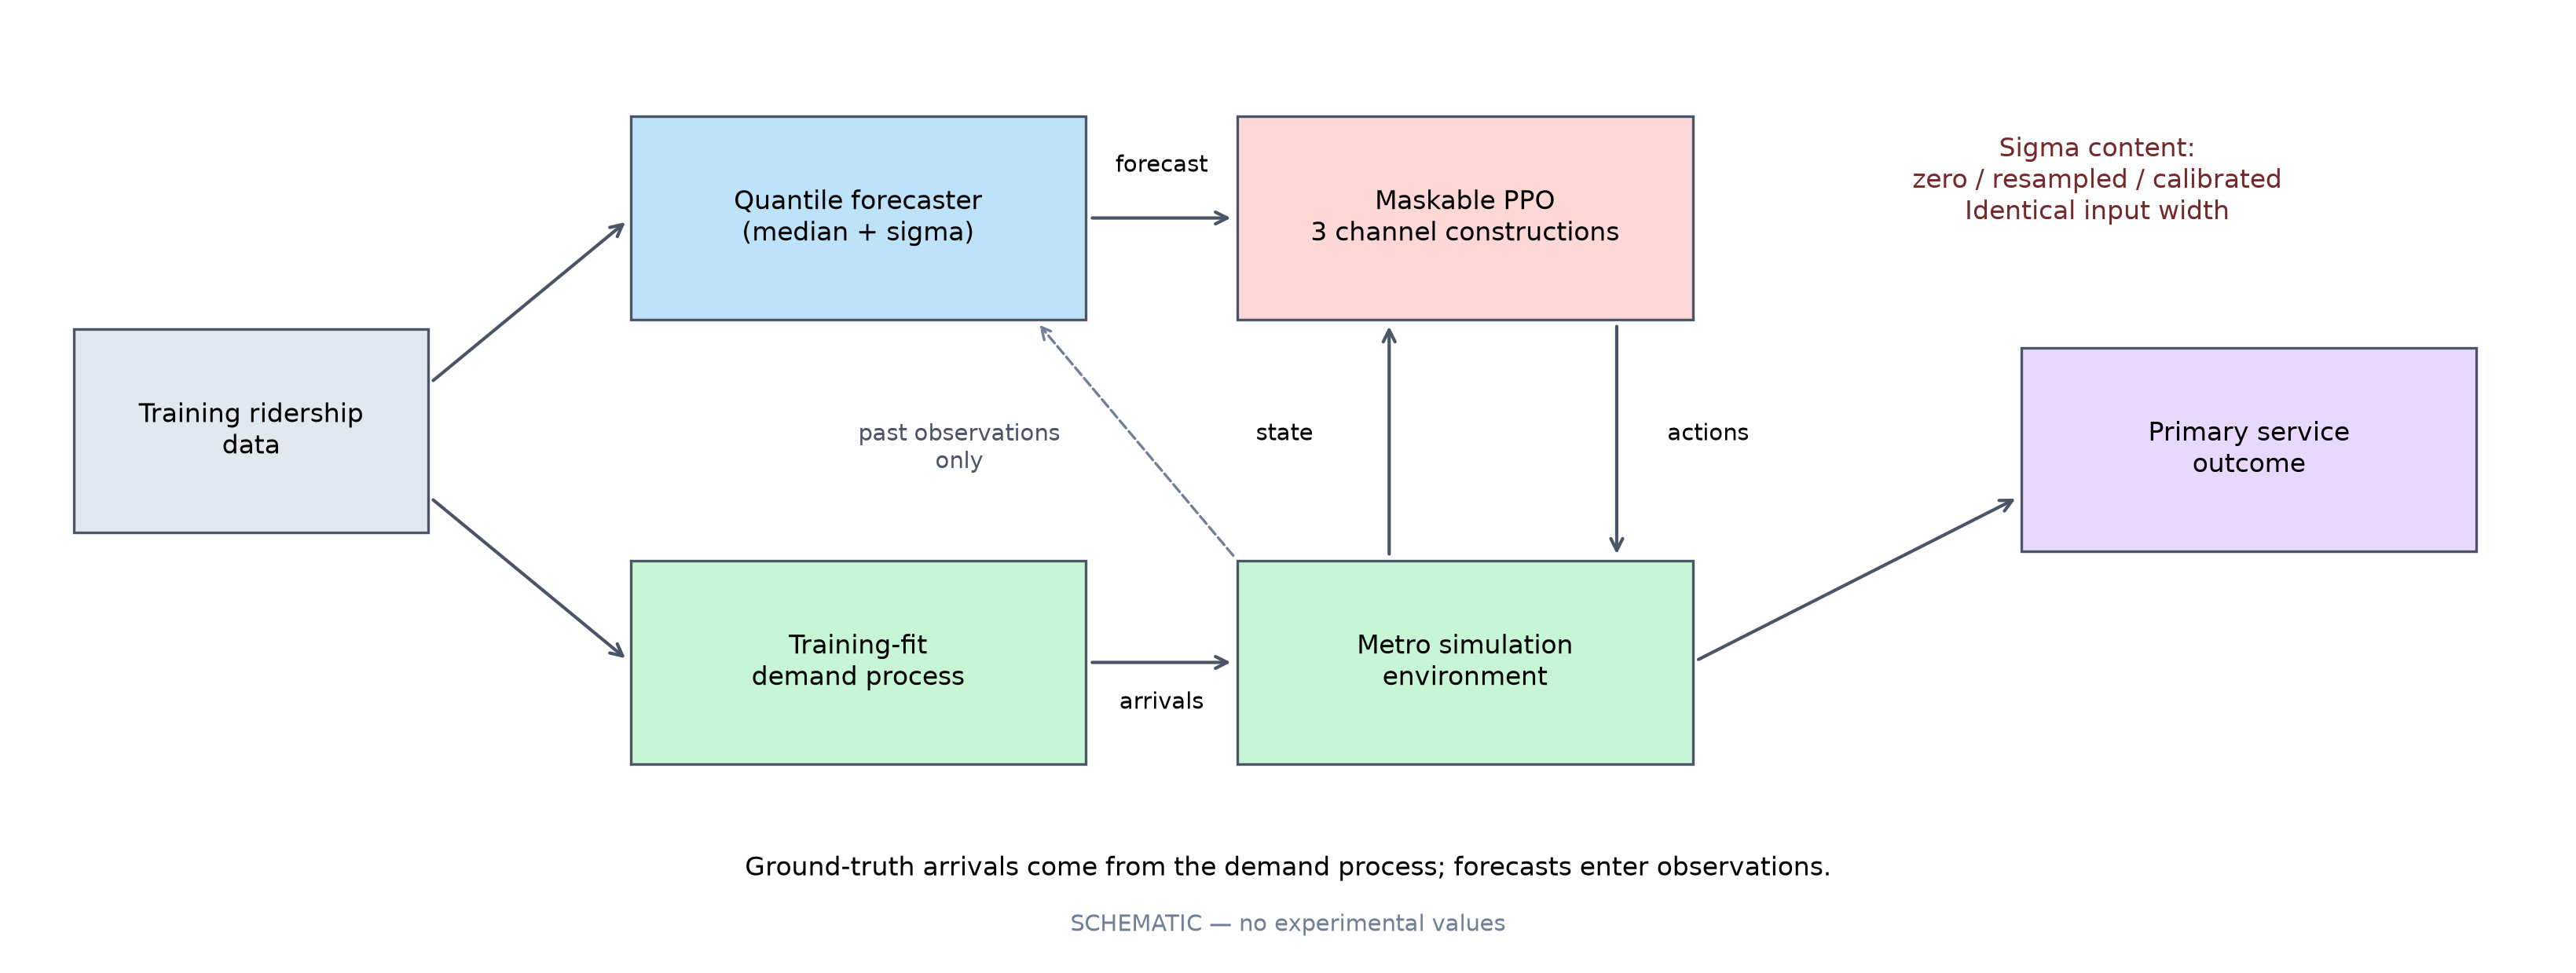
\includegraphics{../results/paper_figures/fig01_research_framework.png}

\subsubsection{Figure 2. twin
architecture}\label{figure-2-twin-architecture}

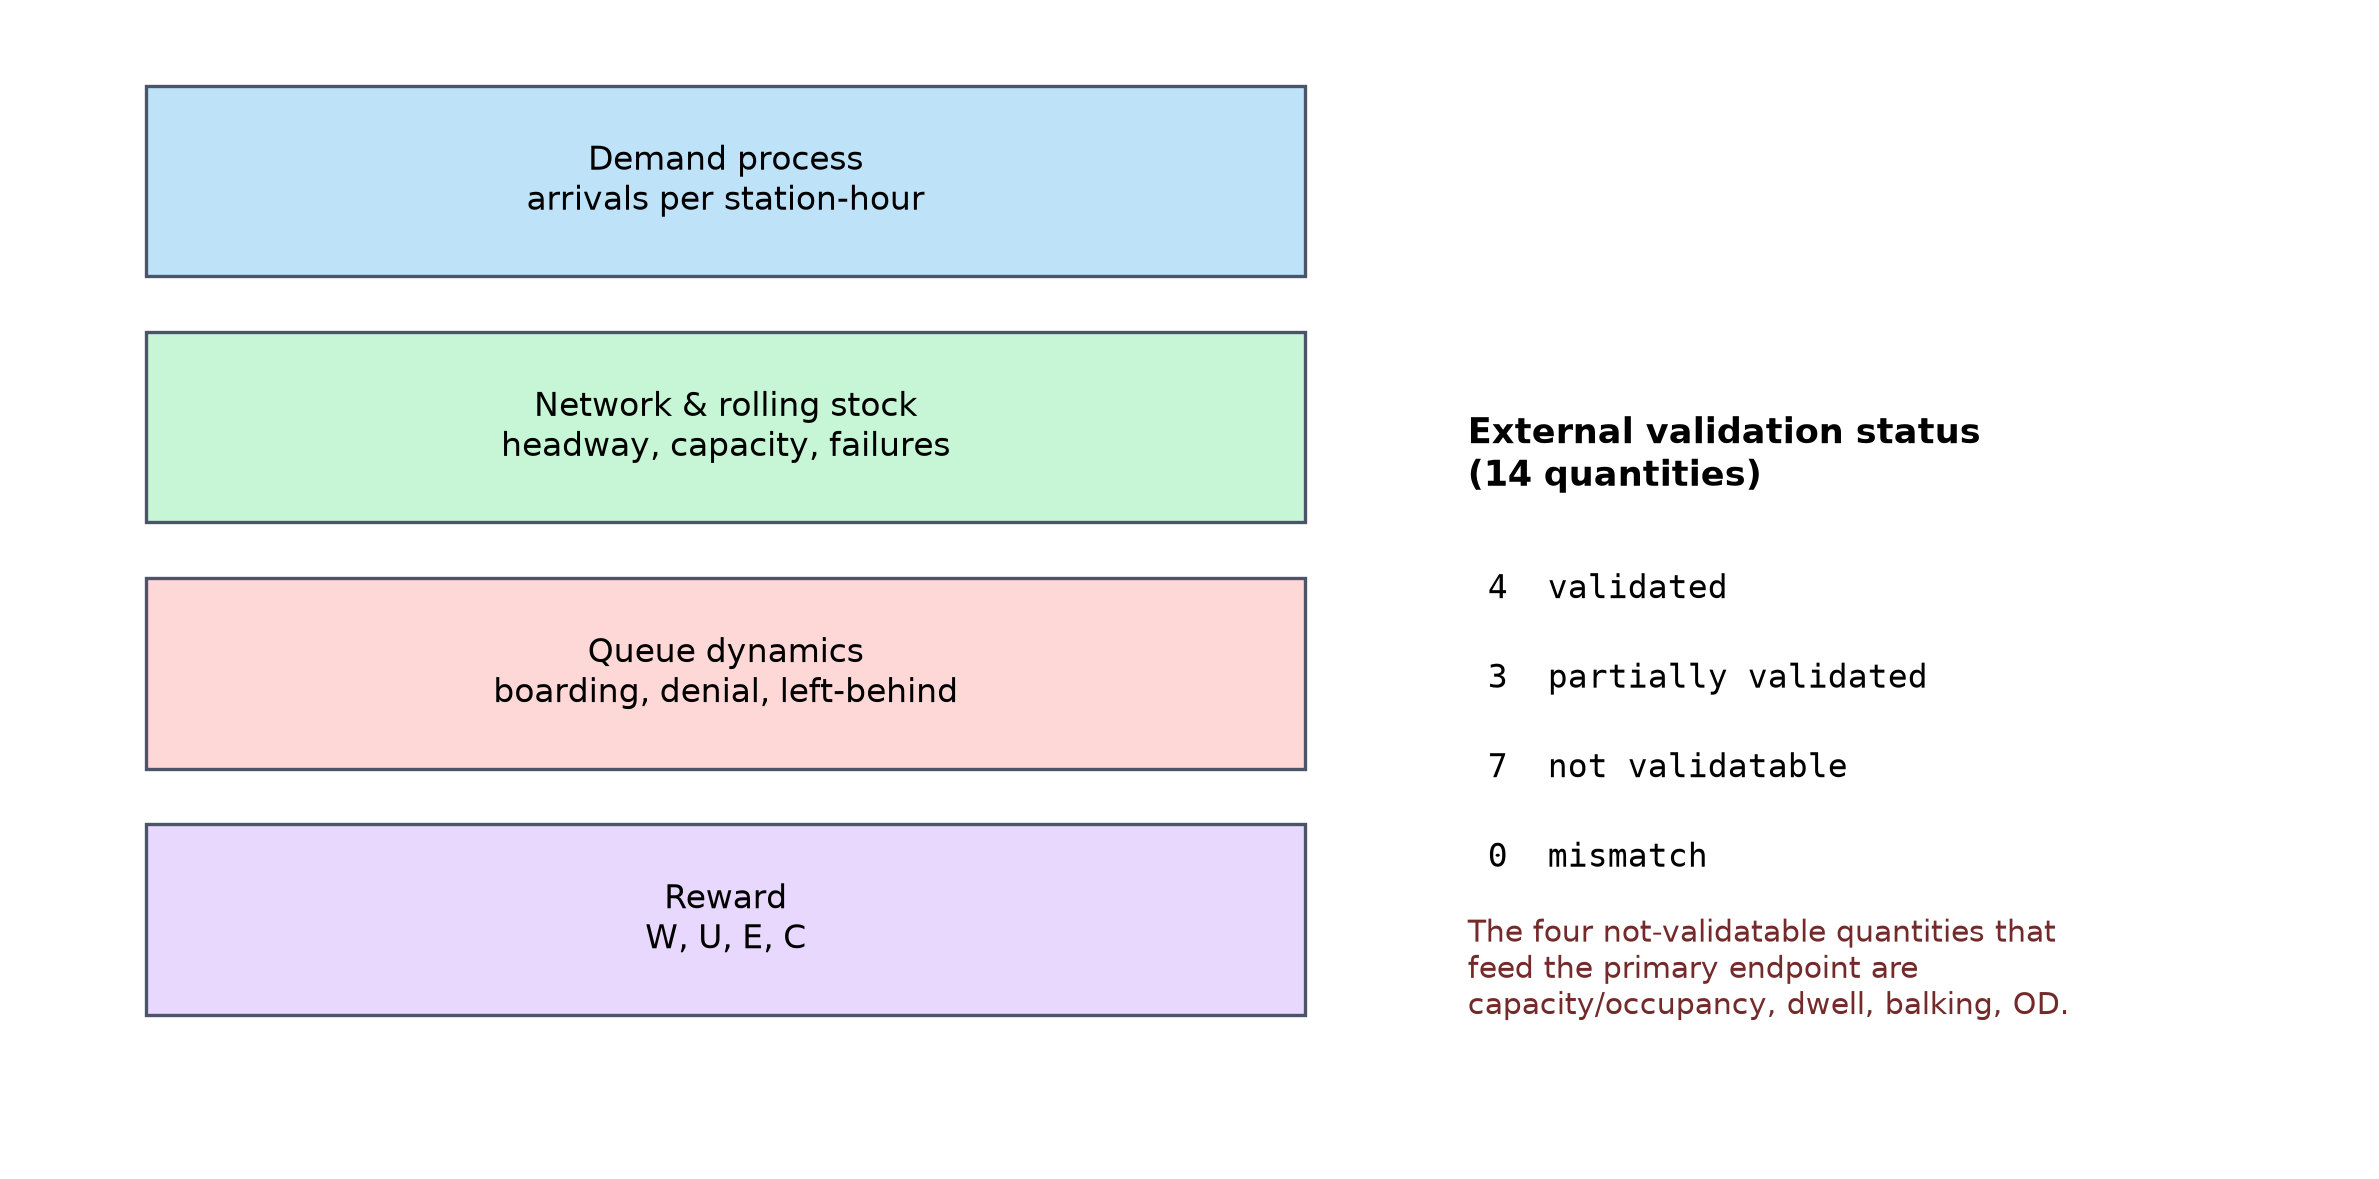
\includegraphics{../results/paper_figures/fig02_twin_architecture.png}

\subsubsection{Figure 3. forecasting}\label{figure-3-forecasting}

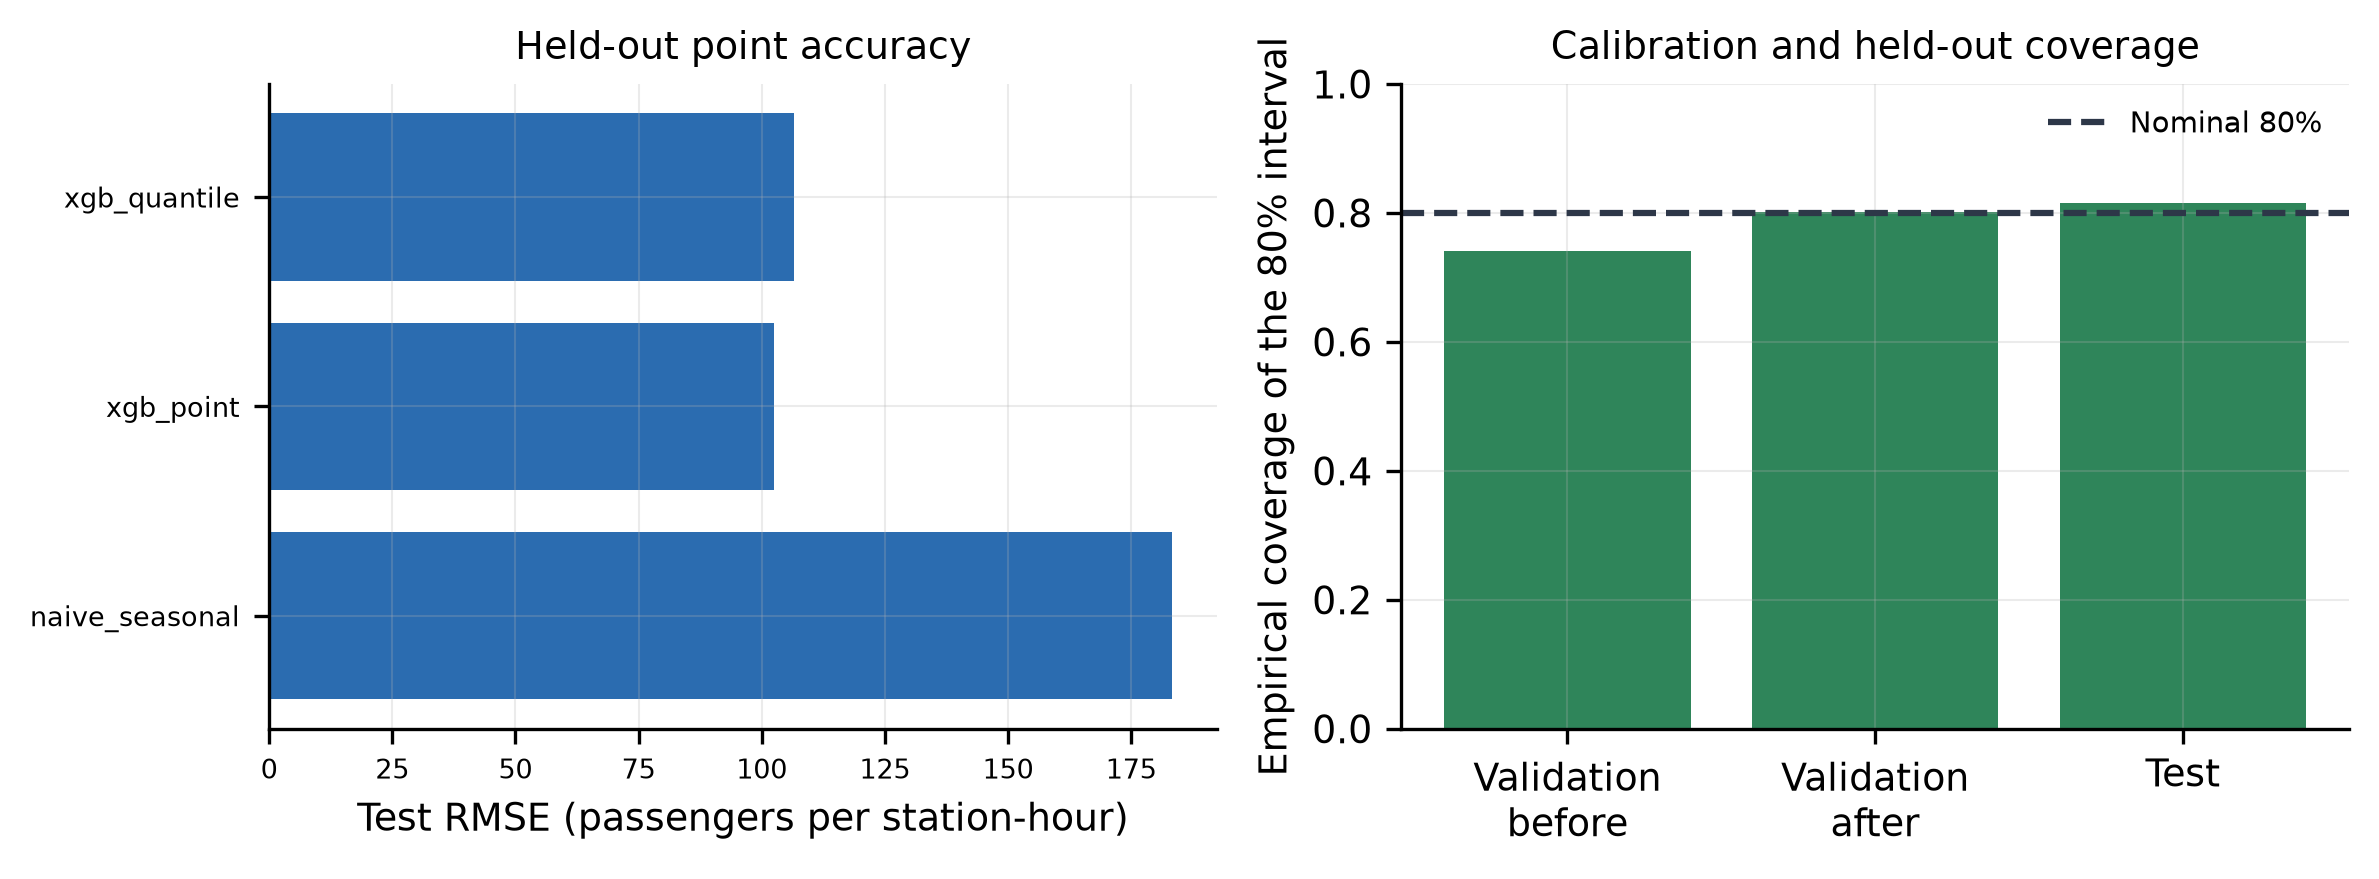
\includegraphics{../results/paper_figures/fig03_forecasting.png}

\subsubsection{Figure 4. primary uq vs
point}\label{figure-4-primary-uq-vs-point}

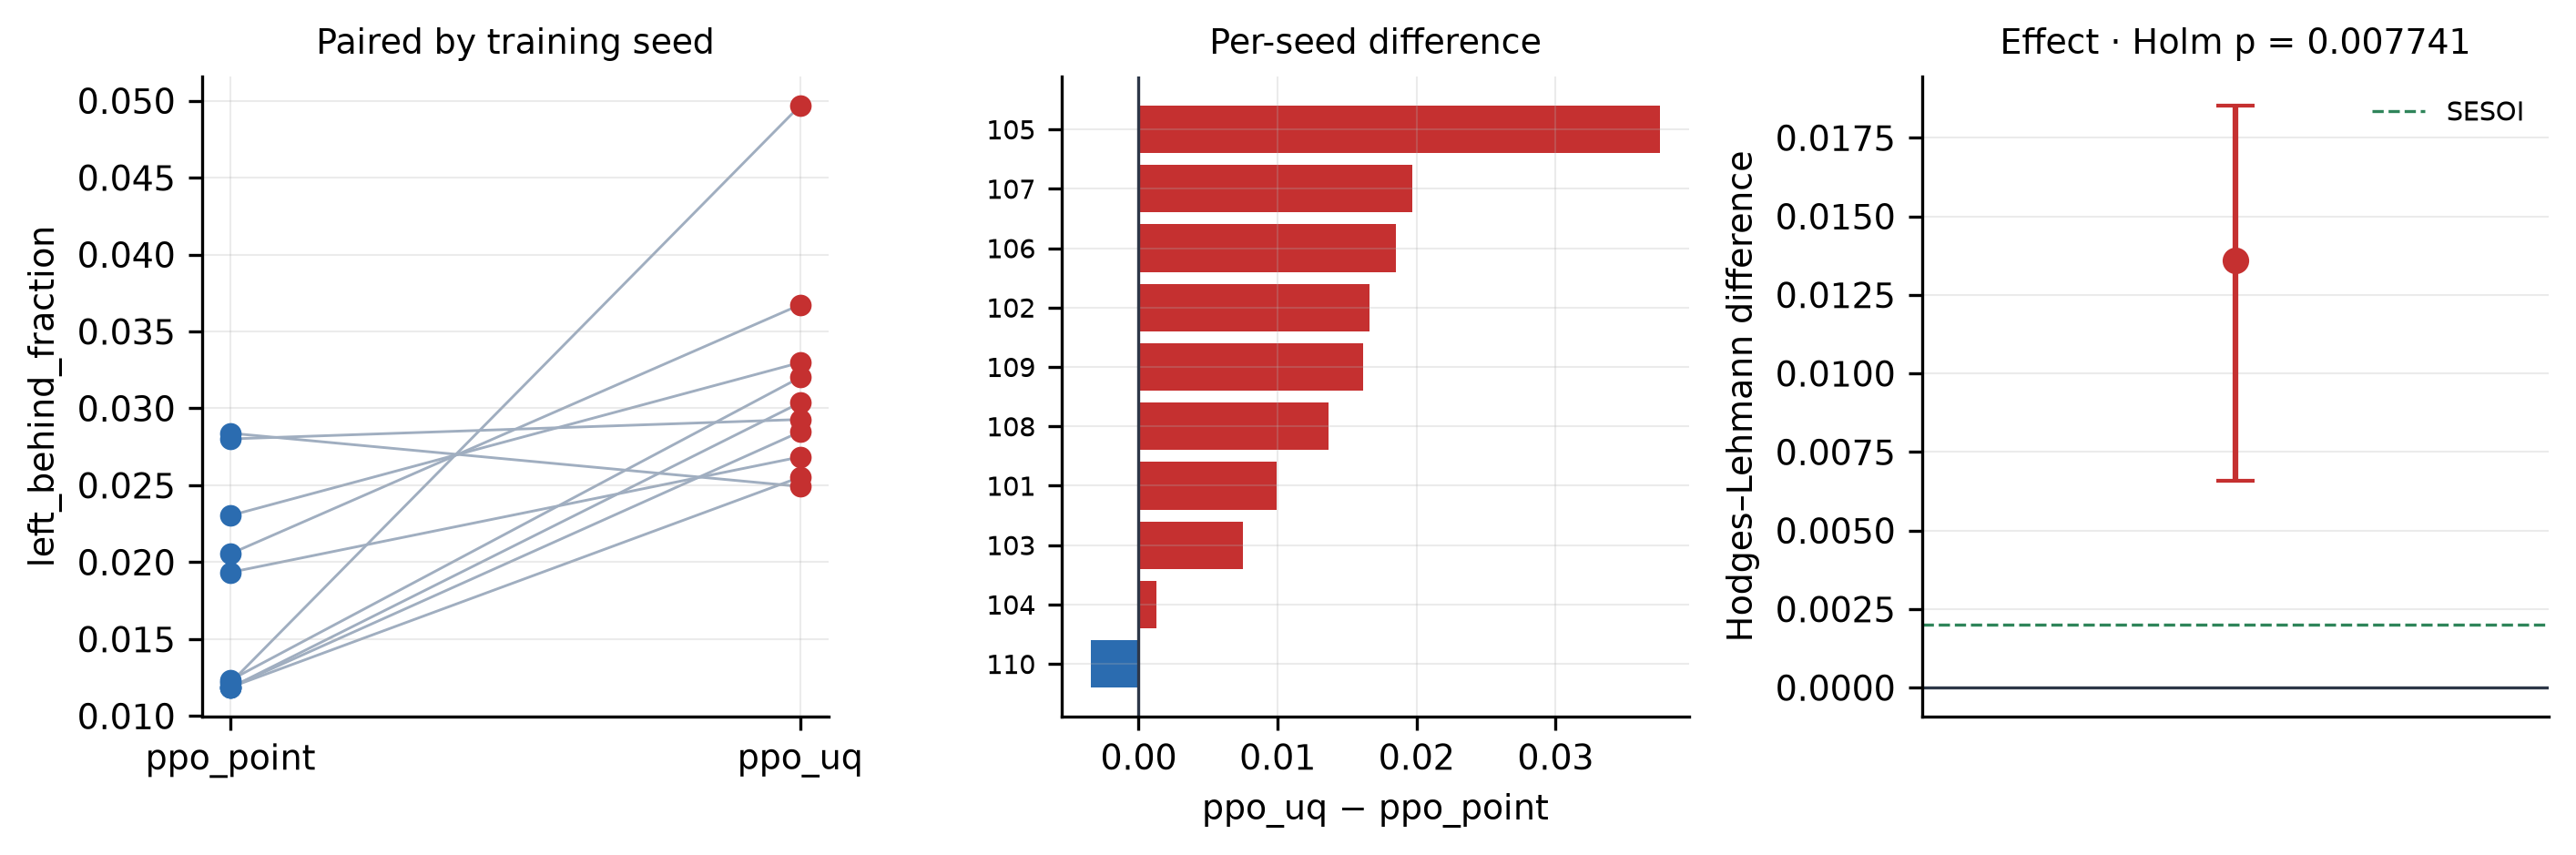
\includegraphics{../results/paper_figures/fig04_primary_uq_vs_point.png}

\subsubsection{Figure 5. placebo}\label{figure-5-placebo}

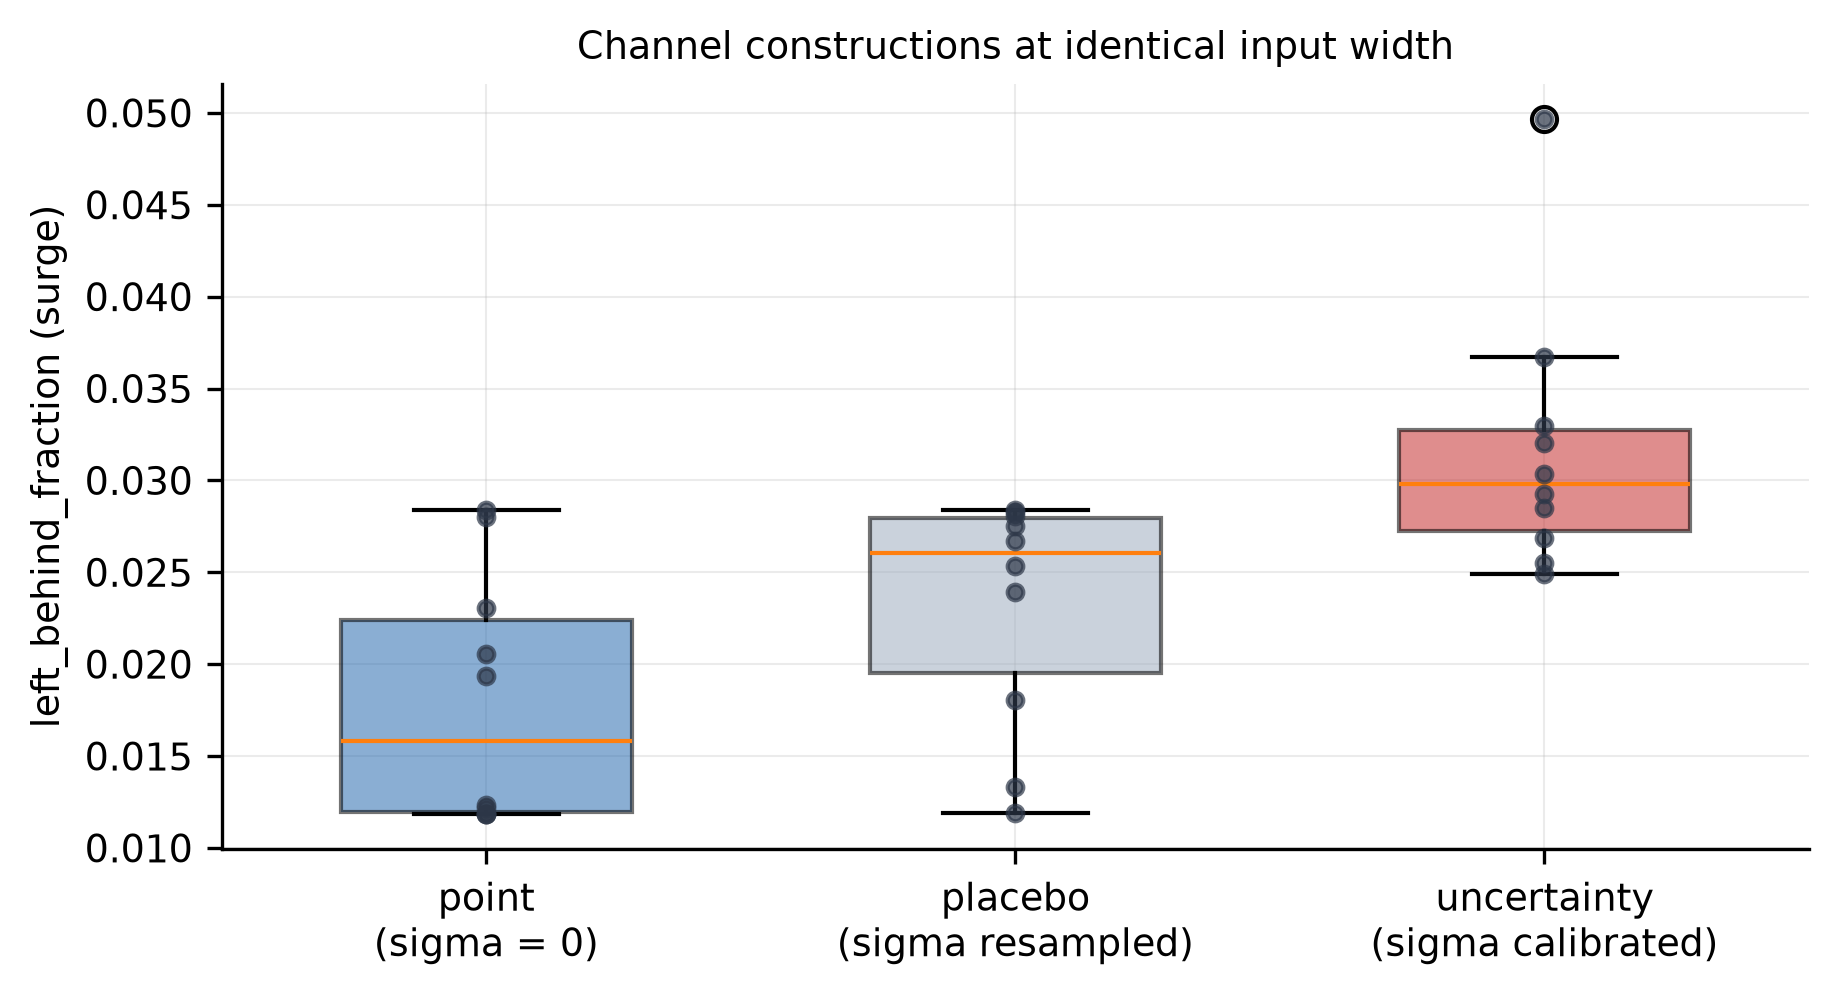
\includegraphics{../results/paper_figures/fig05_placebo.png}

\subsubsection{Figure 6. mechanism}\label{figure-6-mechanism}

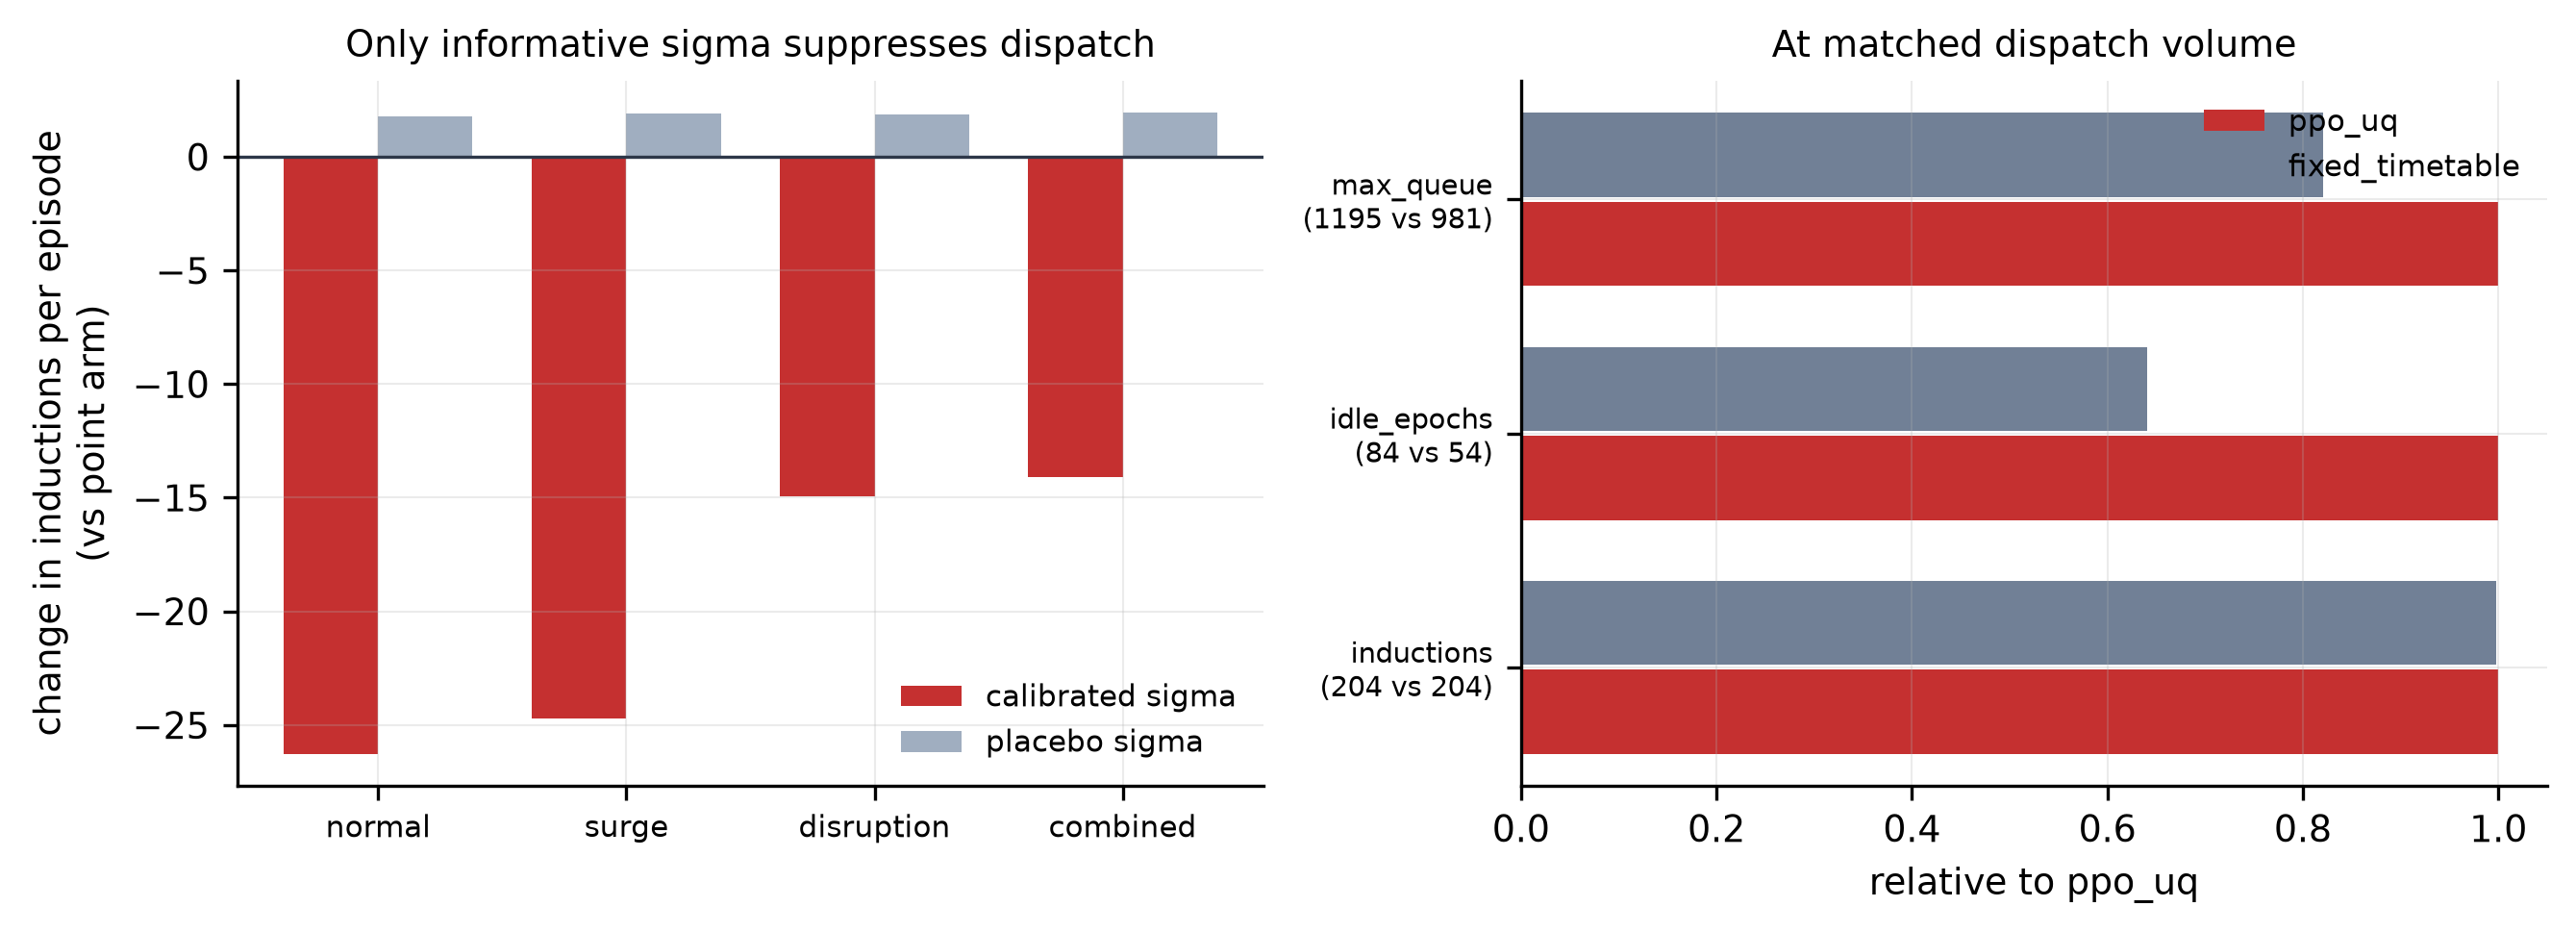
\includegraphics{../results/paper_figures/fig06_mechanism.png}

\subsubsection{Figure 7. Historical arrival/loss curve --- withheld from
this
revision}\label{figure-7-historical-arrivalloss-curve--withheld-from-this-revision}

The archived plot\textquotesingle s epoch-level source data are
unavailable, and its convexity interpretation is not identified by
binned observational summaries. The original file is retained in
results/paper\_figures; it is not presented here as evidence of a
structural loss function.

\subsubsection{Figure 8. scenario
robustness}\label{figure-8-scenario-robustness}

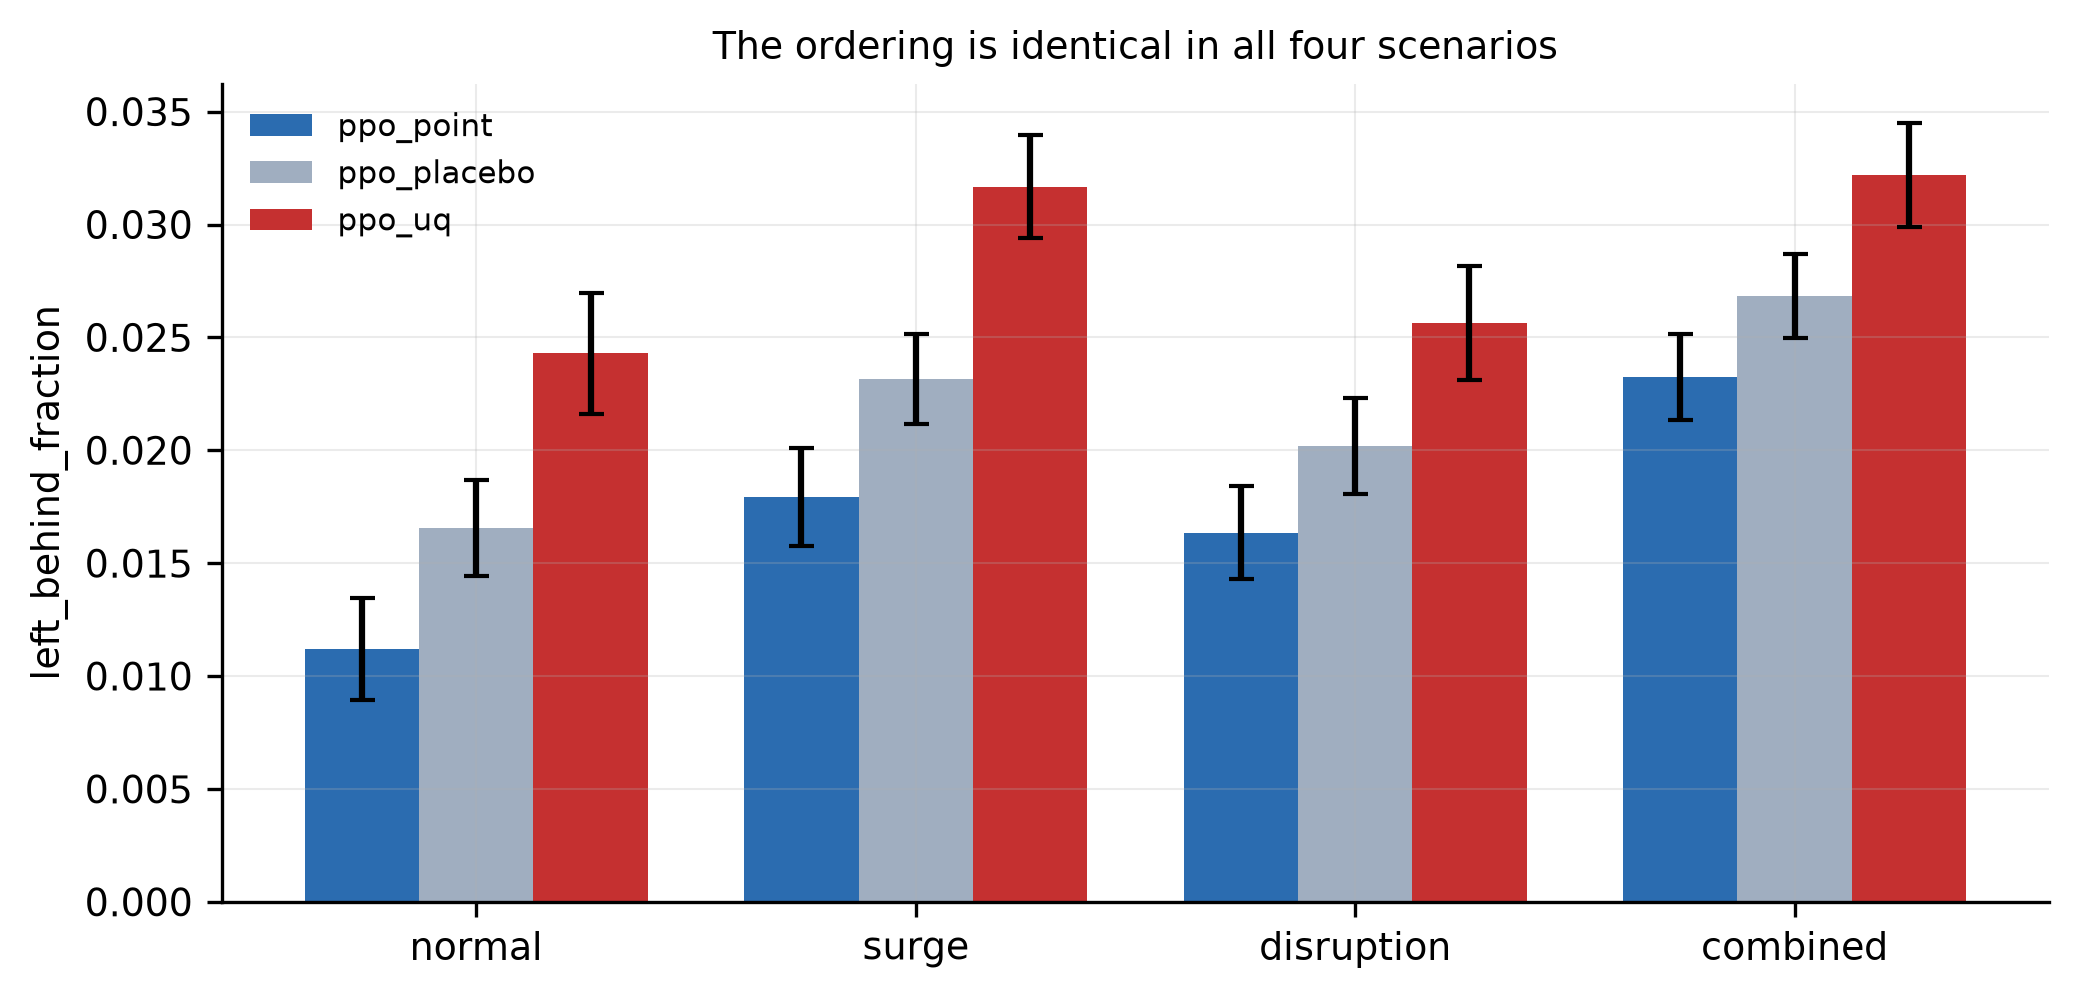
\includegraphics{../results/paper_figures/fig08_scenario_robustness.png}

\subsubsection{Figure 9. baselines}\label{figure-9-baselines}

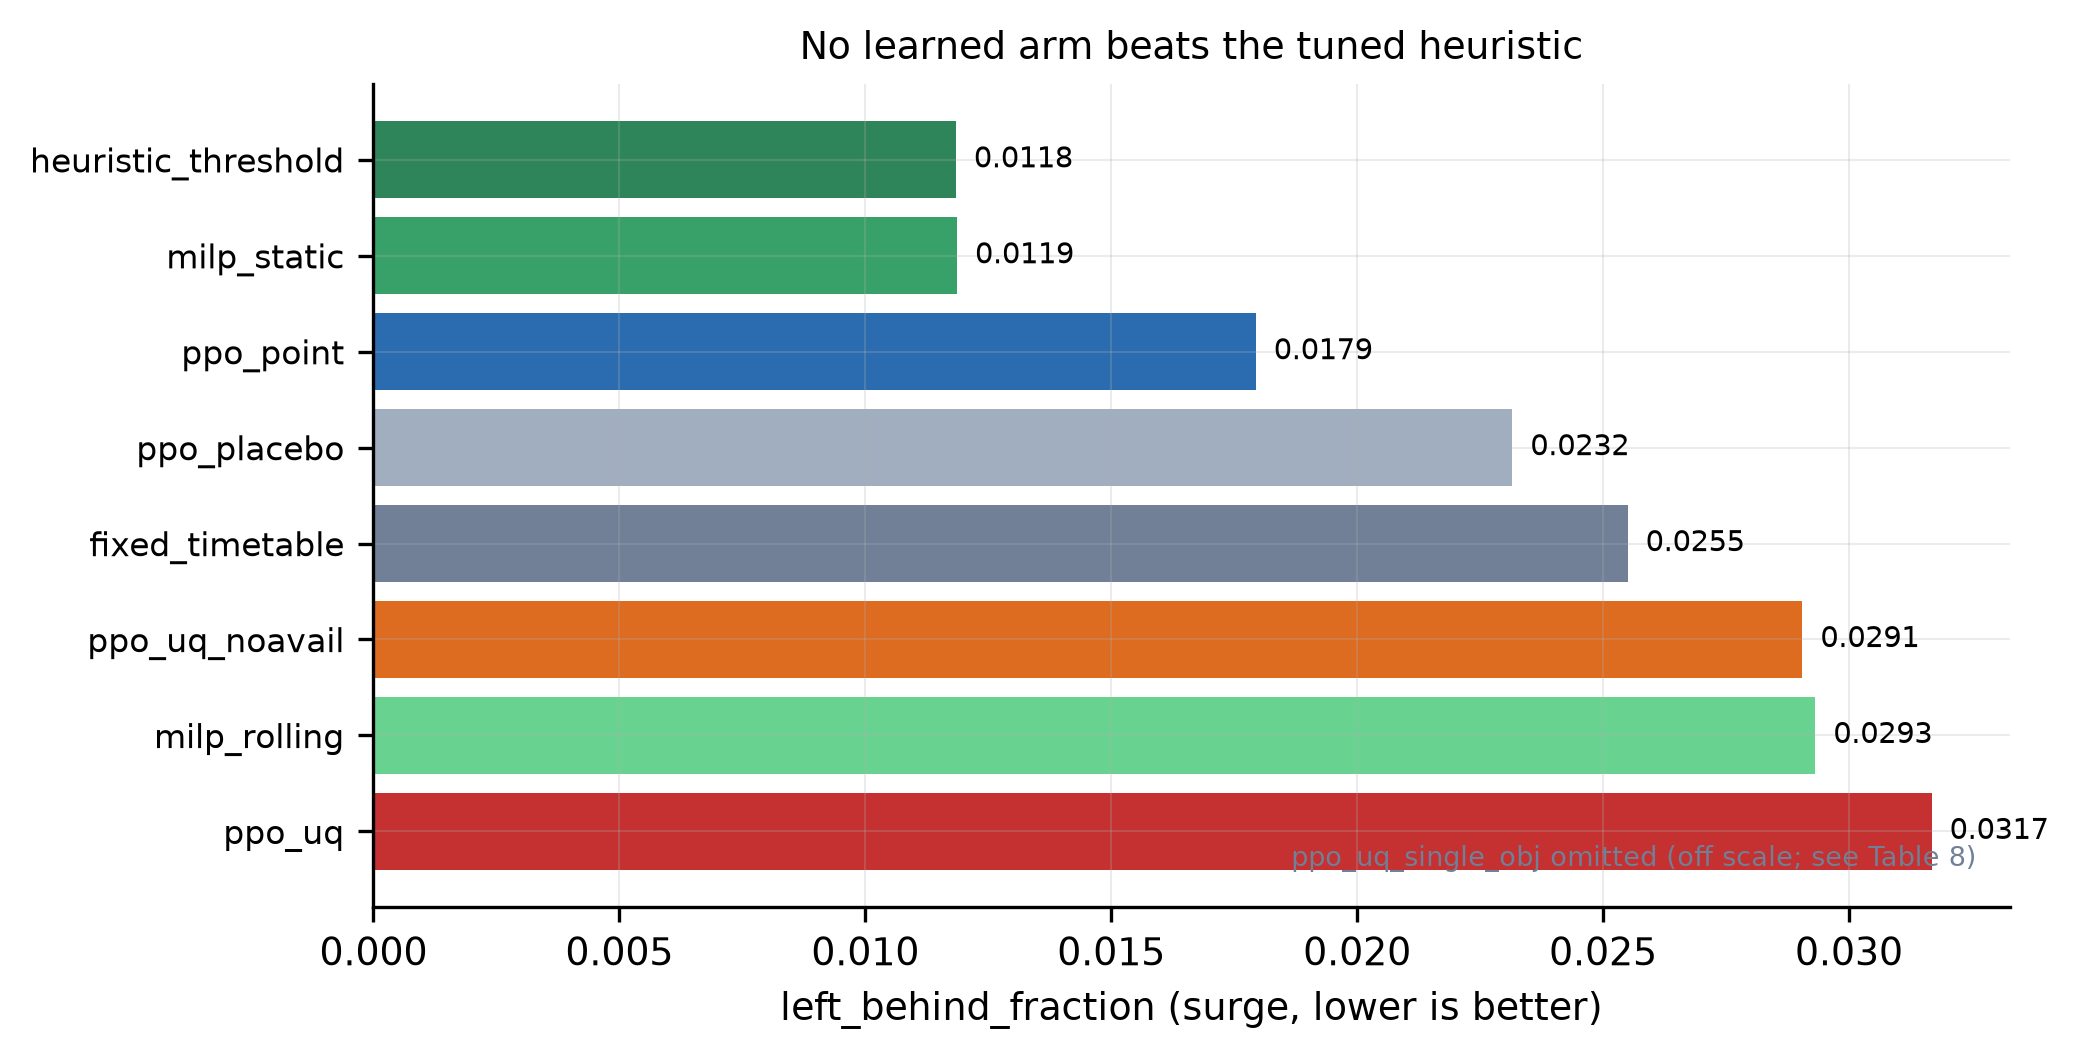
\includegraphics{../results/paper_figures/fig09_baselines.png}

\subsubsection{Figure 10. sensitivity}\label{figure-10-sensitivity}

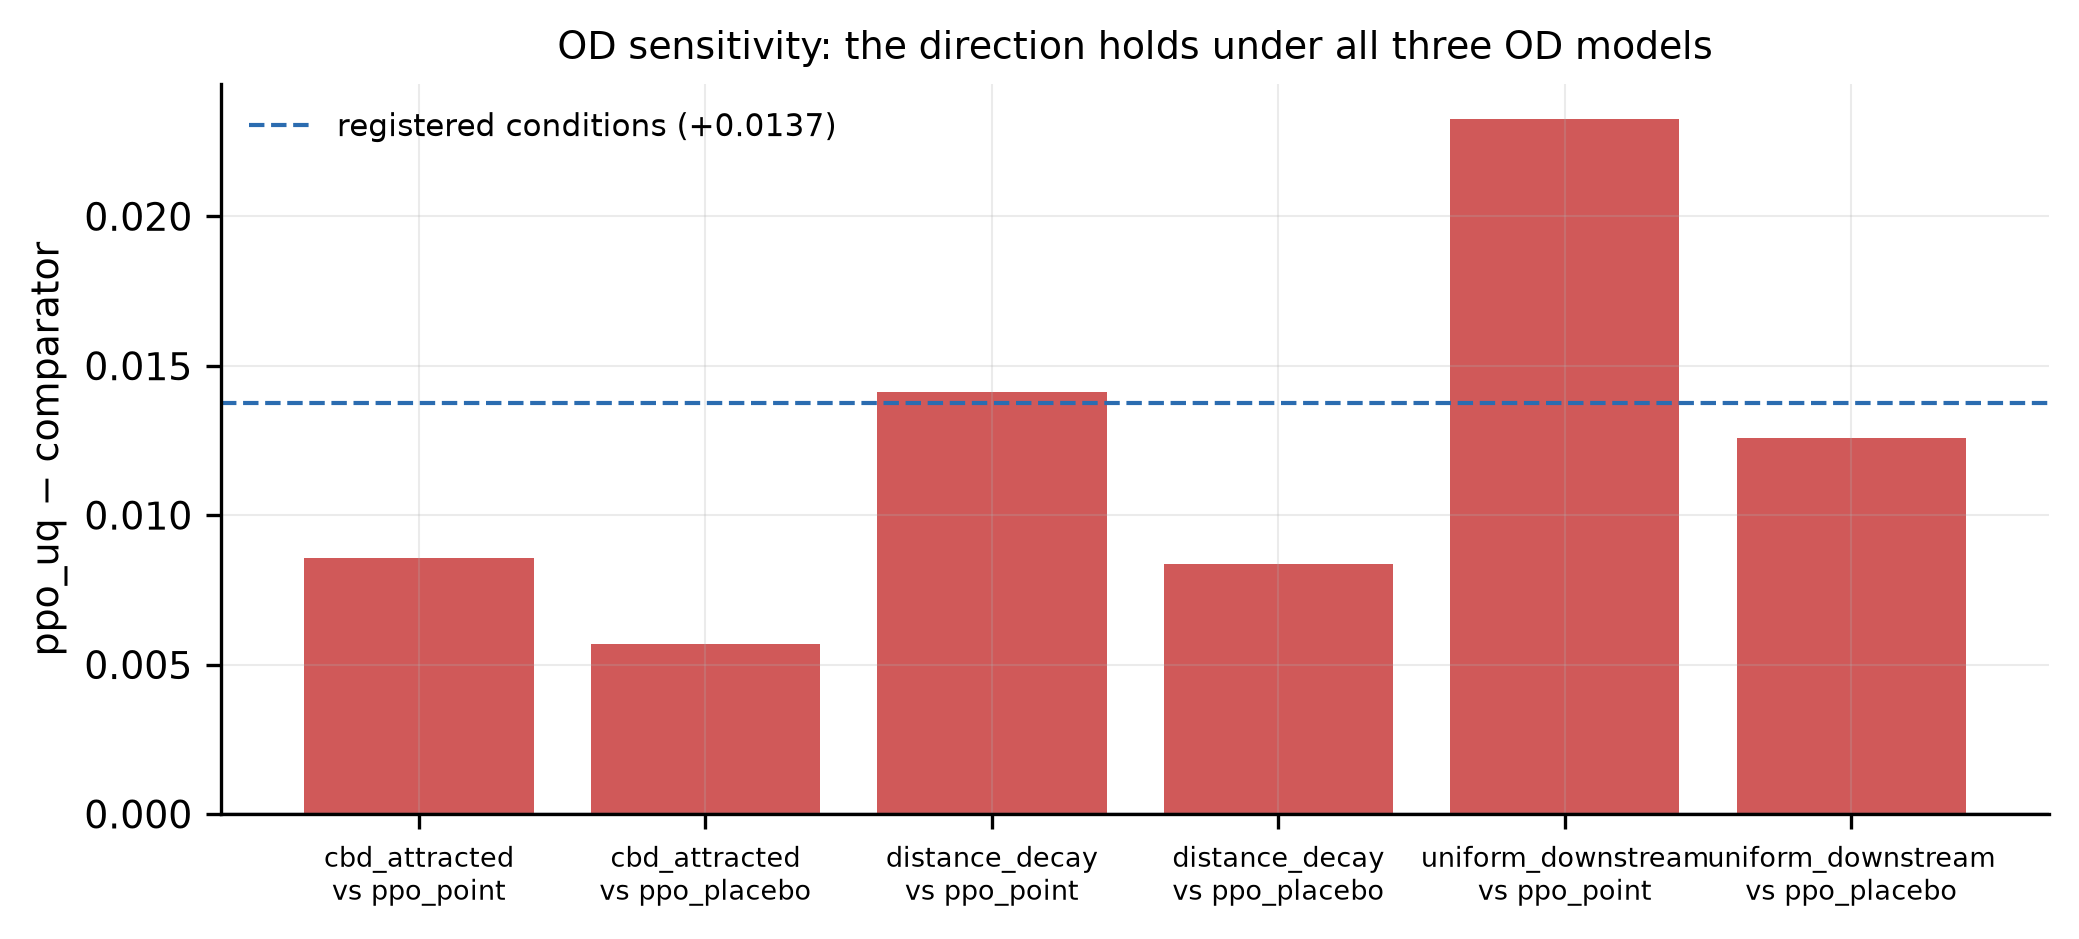
\includegraphics{../results/paper_figures/fig10_sensitivity.png}

\subsubsection{Figure 11. shap}\label{figure-11-shap}

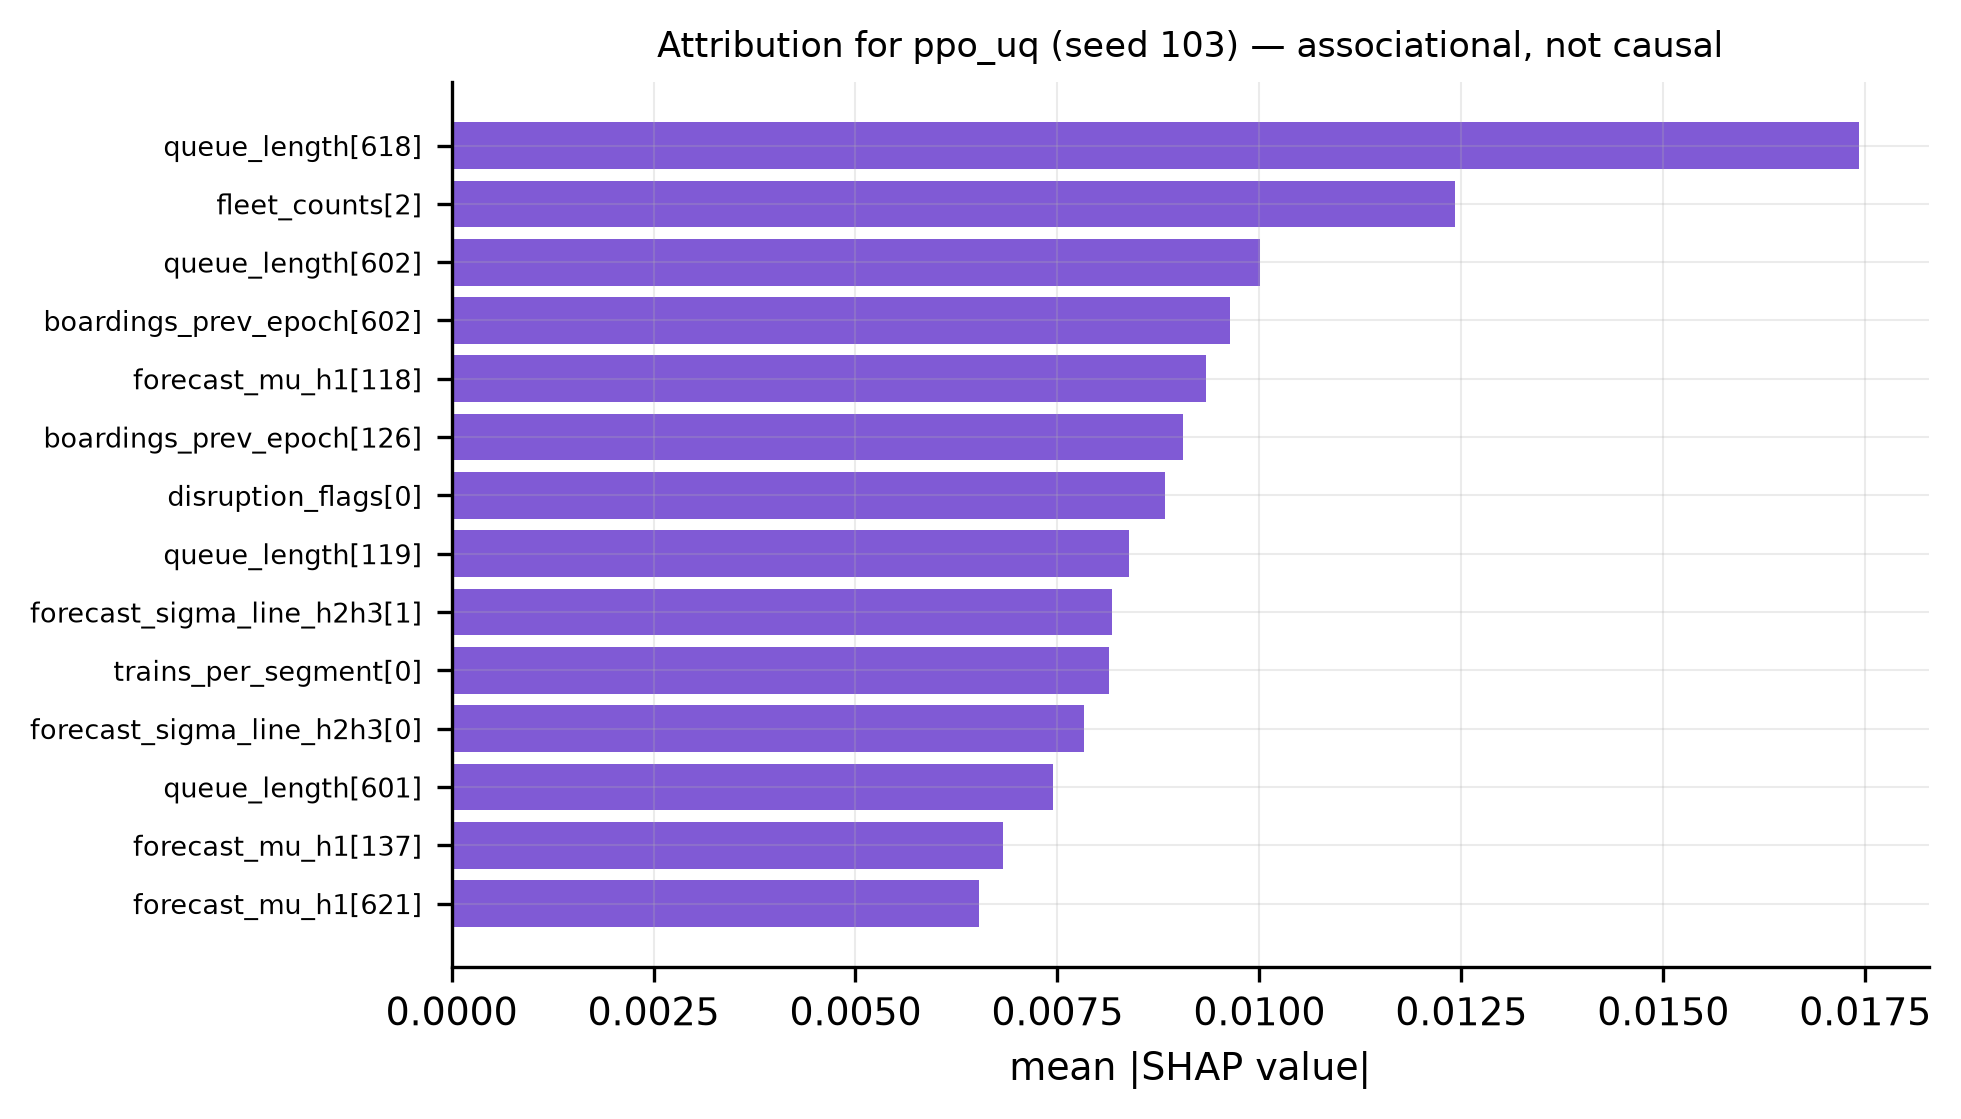
\includegraphics{../results/paper_figures/fig11_shap.png}

\end{document}
